\documentclass{article}
\usepackage{ctex} % 加入ctex宏包以支持中文
\usepackage{graphicx} % 用于插入图片
\usepackage{geometry} % 用于设置页面布局
\usepackage{booktabs} % 用于美化表格
\usepackage{enumitem} % 用于自定义列表格式
\usepackage{lipsum}  % 导入生成段落的宏包
\usepackage{ctex} % 加入ctex宏包以支持中文
\usepackage{graphicx} % 加载图形处理宏包
\usepackage{booktabs} % 用于美化表格线条
\usepackage{caption} % 用于添加表格标题
\usepackage[table]{xcolor} % 用于设置表格颜色
\usepackage{float}

\usepackage{subcaption}
\usepackage{tabularx}
\usepackage{tcolorbox}
\tcbuselibrary{listings}
\usepackage{array}
\usepackage[dvipsnames]{xcolor}
\usepackage{tikz}
\usepackage{hyperref} 
\usepackage{framed}
\usetikzlibrary{positioning} % 加载positioning库
\renewcommand{\refname}{}

\hypersetup{
    colorlinks=true, % 使用颜色而不是边框
    linkcolor=black, % 链接颜色为黑色
    citecolor=black, % 引用颜色为黑色
    urlcolor=blue    % URL颜色为蓝色(可以根据需要修改)
}
\lstset{
 basicstyle=\ttfamily, % 设置字体族
 breaklines=true, % 自动换行
 keywordstyle=\bfseries\color{NavyBlue}, % 设置关键字为粗体,颜色为 NavyBlue
 morekeywords={}, % 设置更多的关键字,用逗号分隔
 emph={self}, % 指定强调词,如果有多个,用逗号隔开
    emphstyle=\bfseries\color{Rhodamine}, % 强调词样式设置
    commentstyle=\itshape\color{black!50!white}, % 设置注释样式,斜体,浅灰色
    stringstyle=\bfseries\color{PineGreen!90!black}, % 设置字符串样式
    columns=flexible,
    % numbers=left, % 显示行号在左边
    % numbersep=2em, % 设置行号的具体位置
    % numberstyle=\footnotesize, % 缩小行号
    % frame=single, % 边框
    framesep=1em, % 设置代码与边框的距离
	tabsize=2, % 设置tab键的宽度为2个空格
    showstringspaces=false, % 不显示字符串中的空格
}

\geometry{a4paper, margin=1in}
\begin{document}

\begin{titlepage}
    \centering
    \vspace*{1cm}

    % 插入学校标志
    
\includegraphics[width=\textwidth]{img/logo.png} % 假设logo.png是学校标志的图片文件

    % \vspace{1.5cm}
    \fontsize{24pt}{32pt}\selectfont
    \textbf{《High-level Language Programming Project》 Report}
    \vspace{4cm}

    \centering
    Ztest: A C++ Unit Testing Framework
    \vspace{2cm}

    \fontsize{16pt}{16pt}\selectfont
    \begin{tabular}{ll}                                                                \\
        School       :   & School of Future Technology\hspace{6cm}          \\
        Major        :   & Data Science and Big Data Technology\hspace{6cm} \\
        Student Name :   & Zheng Chenyang,Ye Suohua,Wu Hongqing,            \\
                         & Qi Yansong,Wang Ruizhen                          \\
        Teacher      :   & Zhang Huaidong\hspace{6cm}                       \\
        Submission Date: & 2025.6.6\hspace{6cm}                             \\
    \end{tabular}

    \vfill

    \vspace{1cm}
\end{titlepage}

\tableofcontents  % 生成目录表
\newpage
\section{System Requirements Analysis}
\subsection{System Background and Motivation}
As the need to cultivate students' complex system architecture design abilities grows, mastering object-oriented design principles and pattern-oriented engineering practices has become a key goal in advanced software engineering education. This requires not only an understanding of the dynamic协作relationship between classes and objects but also the ability to use design patterns to solve architectural problems through abstract thinking.
Existing unit testing frameworks (such as Google Test) have a high learning curve, limited concurrency support, basic reporting systems, and average extensibility. Our team plans to develop a flexible, efficient, and easy-to-use testing tool with a graphical user interface (GUI) to provide an intuitive environment for developers and testers to write, run, and manage test cases. This tool will support various test types (such as unit testing and integration testing) and offer detailed test result reports.
\begin{table}[h]
    \centering
    \caption{Comparison of Mainstream Testing Frameworks}
    \label{tab:compare}
    \begin{tabular}{lccccc}
        \toprule
        \textbf{Framework}    & \textbf{GUI Support} & \textbf{Concurrent Testing} & \textbf{Reporting System} & \textbf{Data-Driven} \\
        \midrule
        gtest (C++)           & None                 & Limited                     & Basic                     & Not Supported        \\
        JUnit (Java)          & Plugin               & Supported                   & HTML/XML                  & Supported            \\
        PyTest (Python)       & Third-Party          & Excellent                   & Rich                      & Supported            \\
        Catch2 (C++)          & None                 & Average                     & Concise                   & Not Supported        \\
        \midrule
        \textbf{Ztest*} (C++) & Excellent            & Excellent                   & Rich                      & Supported            \\
        \bottomrule
    \end{tabular}
\end{table}}
\subsection{System Objectives}
\begin{figure}[H]
    \centering
    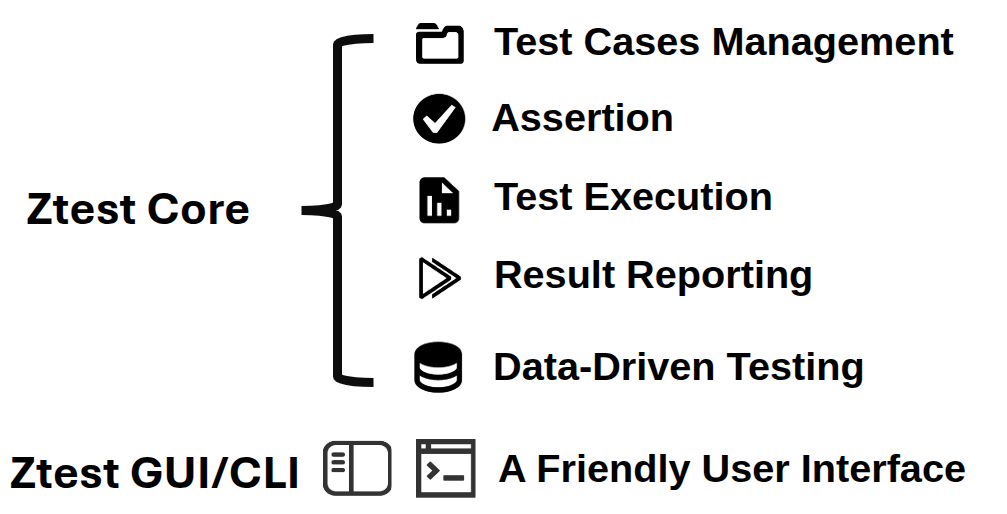
\includegraphics[width=0.6\textwidth]{img/func.png} % 假设logo.png是学校标志的图片文件
    \caption{ Ztest Function}
    \label{fig:ztest function }
\end{figure}
\subsubsection{Test Management}
Compared to traditional unit testing frameworks, Ztest supports various test types, such as thread-safe parallel tests, serial tests, performance evaluation through iteration, and data-driven parameterized tests. We provide test fixtures to manage individual tests.

\begin{figure}[H]
    \centering
    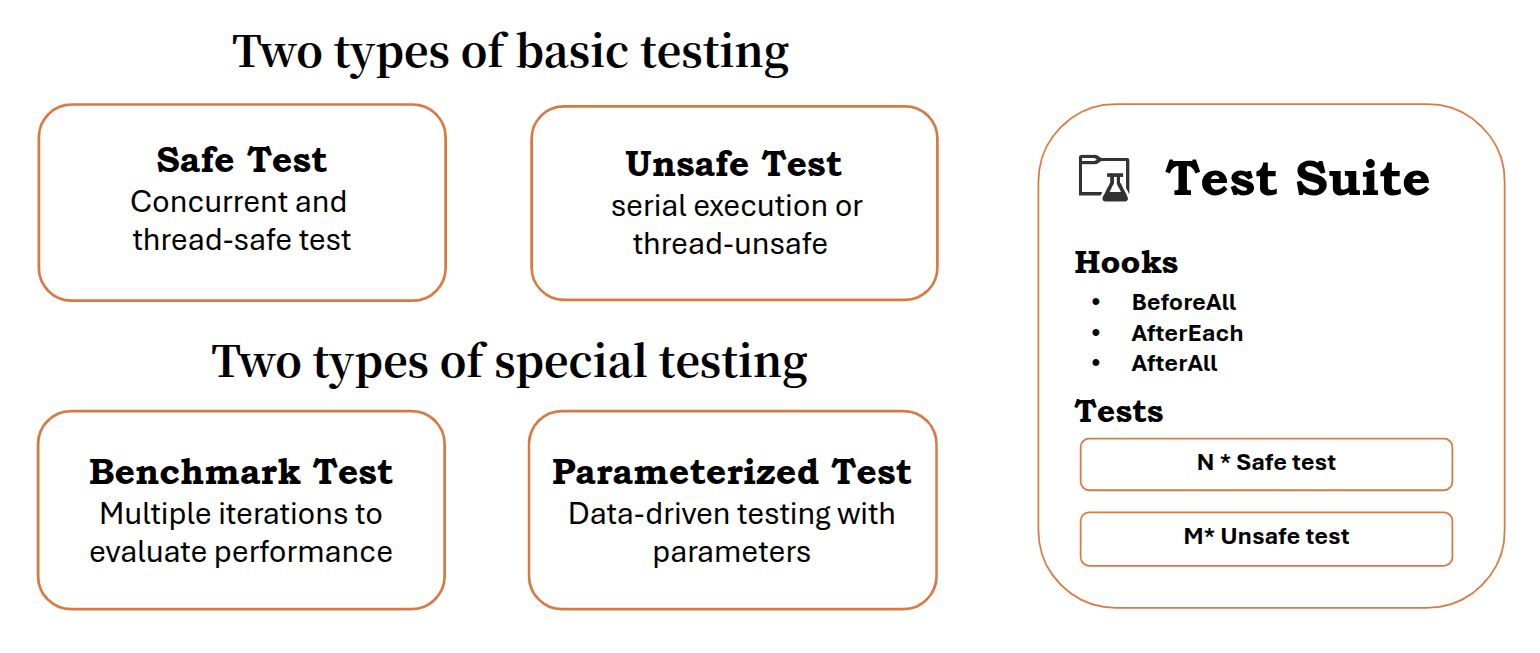
\includegraphics[width=0.8\textwidth]{img/types.png} % 假设logo.png是学校标志的图片文件
    \caption{ Test Type}
    \label{fig:test types }
\end{figure}
We offer macros similar to Google Test to simplify test definition:
\begin{framed}
    \begin{lstlisting}[language=C++]
ZTEST_F(SuiteName, TestName, safe/unsafe) { ... } //define a test 
ZBENCHMARK(SuiteName, TestName, iterations) { ... } // define a benchmark
ZTEST_P(SuiteName, TestName, data) { ... }  //define a parameterized test
ZTEST_P_CSV(SuiteName, TestName, "data.csv") { ... } // define a parameterized test with csv data
\end{lstlisting}
\end{framed}

At the same time, we can define test cases in a chained manner:
\begin{framed}
    \begin{lstlisting}[language=C++]
auto test_case = TestFactory::createTest("Add", ZType::Z_SAFE, "", add, 2, 3)
                 .setExpectedOutput(5)
                 .beforeAll([]() { logger.info("Init\n"); })          
                 .afterEach([]() { logger.info("Clean\n"); }).build();
                \end{lstlisting}
\end{framed}

\subsubsection{Assertion Mechanism}
The assertion mechanism is used to verify whether the expected results of test cases are correct. The framework provides various assertion macros, such as \textbf{EXPECT\_EQ} and \textbf{ASSERT\_TRUE}, to quickly validate conditions in tests.
The main assertions provided are:
\begin{itemize}
    \item \textbf{EXPECT\_EQ}: Verifies whether two values are equal.
    \item \textbf{ASSERT\_TRUE}: Verifies whether a condition is true.
\end{itemize}
Usage example:
\begin{lstlisting}[language=C++]
// If the assertion fails, an exception is thrown
EXPECT_EQ(5, add(2, 3));
ASSERT_TRUE(6==add(2, 3));
\end{lstlisting}

If an assertion fails, a \textbf{ZTestFailureException} is thrown. Custom exception handling logic can also be implemented by inheriting from \textbf{ZTestFailureException}.
\subsubsection{Data-Driven Testing}
Parameterized testing involves replacing certain fixed data in test cases with parameters and generating multiple sets of test data by changing the parameter values to test the software multiple times. It allows testers to cover multiple input scenarios with a single set of test logic instead of writing separate test code for each scenario.
ZTest implements parameterized testing and uses CSV import and data parsing to achieve data-driven testing. To accelerate data access, imported data is cached. A lazy loading mechanism is employed, where data is only loaded into the cache when needed, reducing unnecessary resource consumption. Additionally, an LRU cache eviction strategy is used to ensure that the cached data is the most likely to be accessed again, thereby maximizing the effectiveness of the cache.

\subsubsection{Test Executor}
The test executor is responsible for managing the execution of test cases, supporting \textbf{concurrent} execution of test cases, and collecting test results, achieving automatic scheduling of tests and test result statistics.
Its behavior is as follows:
\begin{itemize}
    \item Run safe tests in parallel. Thread creation and destruction are relatively time-consuming operations. Using a thread pool to manage the lifecycle of threads avoids frequent thread creation and destruction, thereby significantly improving system performance.
    \item Run unsafe tests in sequence. A queue is used to maintain test cases to ensure ordered execution.
    \item Run Benchmark tests in sequence.
    \item Run Parameterized tests in sequence.
\end{itemize}
\subsubsection{Report Generation}
It can generate HTML, JSON, and XML reports for easy viewing of test results and integration with CI/CD.
\begin{figure}[H]
    \centering
    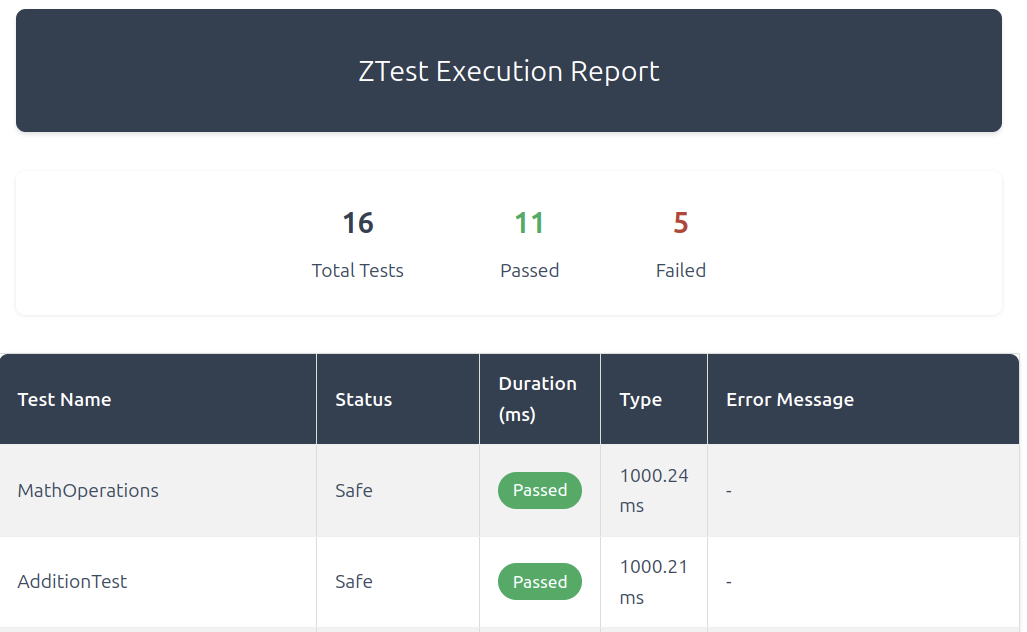
\includegraphics[width=0.8\textwidth]{img/report.png}
    \caption{Test Result Display Interface Layout Diagram}
    \label{fig:report}
    \small
\end{figure}
\subsubsection{CLI Interface}
\begin{framed}
    \begin{lstlisting}
Usage: executor_name [OPTIONS] 
Options: 
--help                         Show help 
--run-all                      Run all tests
--run-safe                     Run safe tests
--run-unsafe                   Run unsafe tests
--run-benchmark                Run benchmark tests
--run-parameterized            Run parameterized tests
--run-test-case TEST_CASE      Run a specific test case
\end{lstlisting}
\end{framed}

\subsubsection{GUI Display}
The GUI can display test results, filter test outcomes, monitor system resource status, and view details of test execution.
\begin{figure}[H]
    \centering
    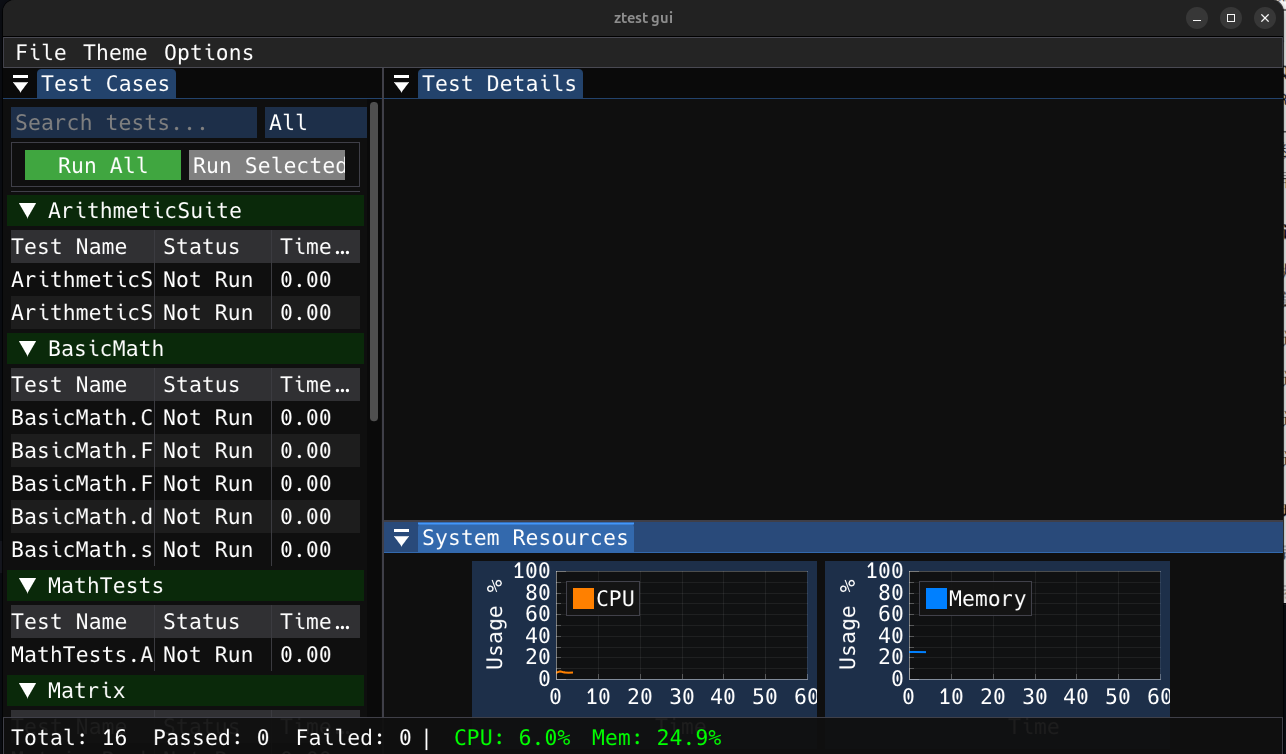
\includegraphics[width=\textwidth]{img/gui.png}
    \caption{Test Management Interface Layout Diagram}
    \label{fig:gui}
    \small
\end{figure}
\subsubsection{AI Intelligent Diagnosis Function}
By calling the qwen3 API, intelligent diagnosis functionality is achieved. Specific analysis of individual test cases can be obtained on the GUI interface. The report will include
\begin{enumerate}
    \item Identifying the root cause of failures
    \item Providing troubleshooting suggestions
    \item Highlighting high-risk test cases
    \item Evaluating overall test coverage
    \item Proposing suggestions for improving system stability
\end{enumerate}
\newpage
\section{Program Analysis}
\subsection{Key System Issues}
\subsubsection{Improving Test Execution Efficiency}
Traditional C++ testing frameworks (such as gtest and catch2) often use sequential test execution, leading to long testing times and reduced productivity. Vibro coding has reduced the time required to write test cases, but the time to run them remains largely unchanged.
We categorize tasks into four types: short testing time with a focus on result accuracy, such as addition operations, string concatenation, and user login validation; long testing time with a focus on result accuracy, such as merging multiple files, complex string matching and replacement, and large data sorting result validation; short testing time with a focus on process evaluation, such as reading or writing large files, low-complexity algorithm performance testing, and database queries; and long testing time with a focus on process evaluation, such as multi-threaded task processing, stress testing, and high-time-complexity algorithm testing.
\begin{figure}[H]
    \centering
    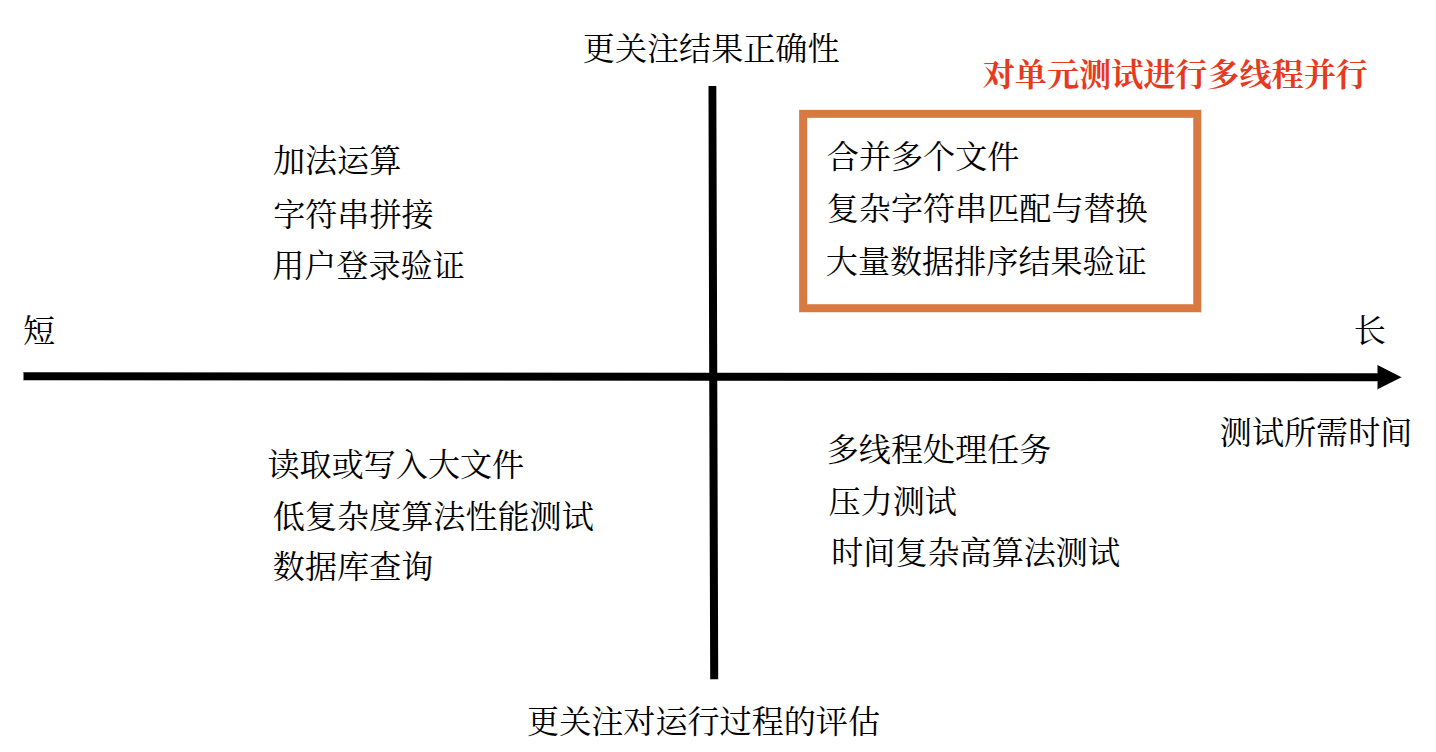
\includegraphics[width=0.8\textwidth]{img/task.png} % 假设logo.png是学校标志的图片文件
    \caption{ Task Type}
    \label{fig:task types }
\end{figure}
For tasks with long testing times that focus on result accuracy and are thread-safe, ZTest introduces multi-threaded test execution directly into the C++ testing framework, rather than relying on third-party tools like google-parallel, achieving finer-grained control.
Additionally, data-driven testing and caching have been introduced to significantly improve the definition and execution speed of large-scale unit tests.
\subsubsection{Syntax Sugar Implementation}
How can we encourage developers to use unit testing frameworks? The key lies in the simplicity of the syntax. We employ a series of complex macro definitions to achieve syntax sugar, thereby simplifying user definitions.
\subsubsection{Automatic Type Inference of Functions to be Tested}
When defining individual test cases using a chained approach, we aim for users to only need to provide the function name, parameters, and expected results, allowing our framework to handle the test execution logic and result verification. This requires automatic inference of the parameter types of the function under test to facilitate function calls for testing and result validation. We utilize the factory pattern to specify the return type and the builder pattern to construct parameters and set expected results.
\subsection{Responsibility Allocation}
\begin{itemize}[leftmargin=*]
    \item Zheng Chenyang: Architecture design, main code writing for ztest core and gui, report writing, and presentation
    \item Ye Suohua: GUI improvement and partial test logic enhancement
    \item Wu Hongqing: GUI improvement
    \item Qi Yansong: GUI improvement
    \item Wang Ruizhen: Attempt to migrate to Windows
\end{itemize}

\section{Technical Approach}
\subsection{Runtime Environment}
\begin{table}[H]
    \centering
    \caption{Development and Operating Environment}
    \begin{tabular}{@{}>{\bfseries}c>{\raggedright\arraybackslash}p{10cm}@{}} % Set the first column to bold and the second column to left-aligned
        \toprule
        \textbf{Component}      & \textbf{Tool Used for Development}                    \\
        \midrule
        Processor               & Intel i9-14900HX (32) @ 5.800GHz                      \\
        Operating System        & Ubuntu 24.04.2 LTS x86\_64 (kernel 6.11.0-26-generic) \\
        Compiler                & gcc 13.3.0 or clang 18.1.3 (MSVC cannot be used)      \\
        Graphics API            & glfw 3.4 + glad 4.0.1                                 \\
        GUI Framework           & ImGui-1.91.7-docking                                  \\
        Data Visualization Tool & implot v0.16                                          \\
        Build System            & XMake v2.9.9+HEAD.40815a0                             \\
        C++ Standard            & C++20 (required)                                      \\
        \bottomrule
    \end{tabular}
\end{table}
\subsection{Overall Design}
\subsubsection{Ztest Core Architecture Diagram}
\begin{figure}[H]
    \centering
    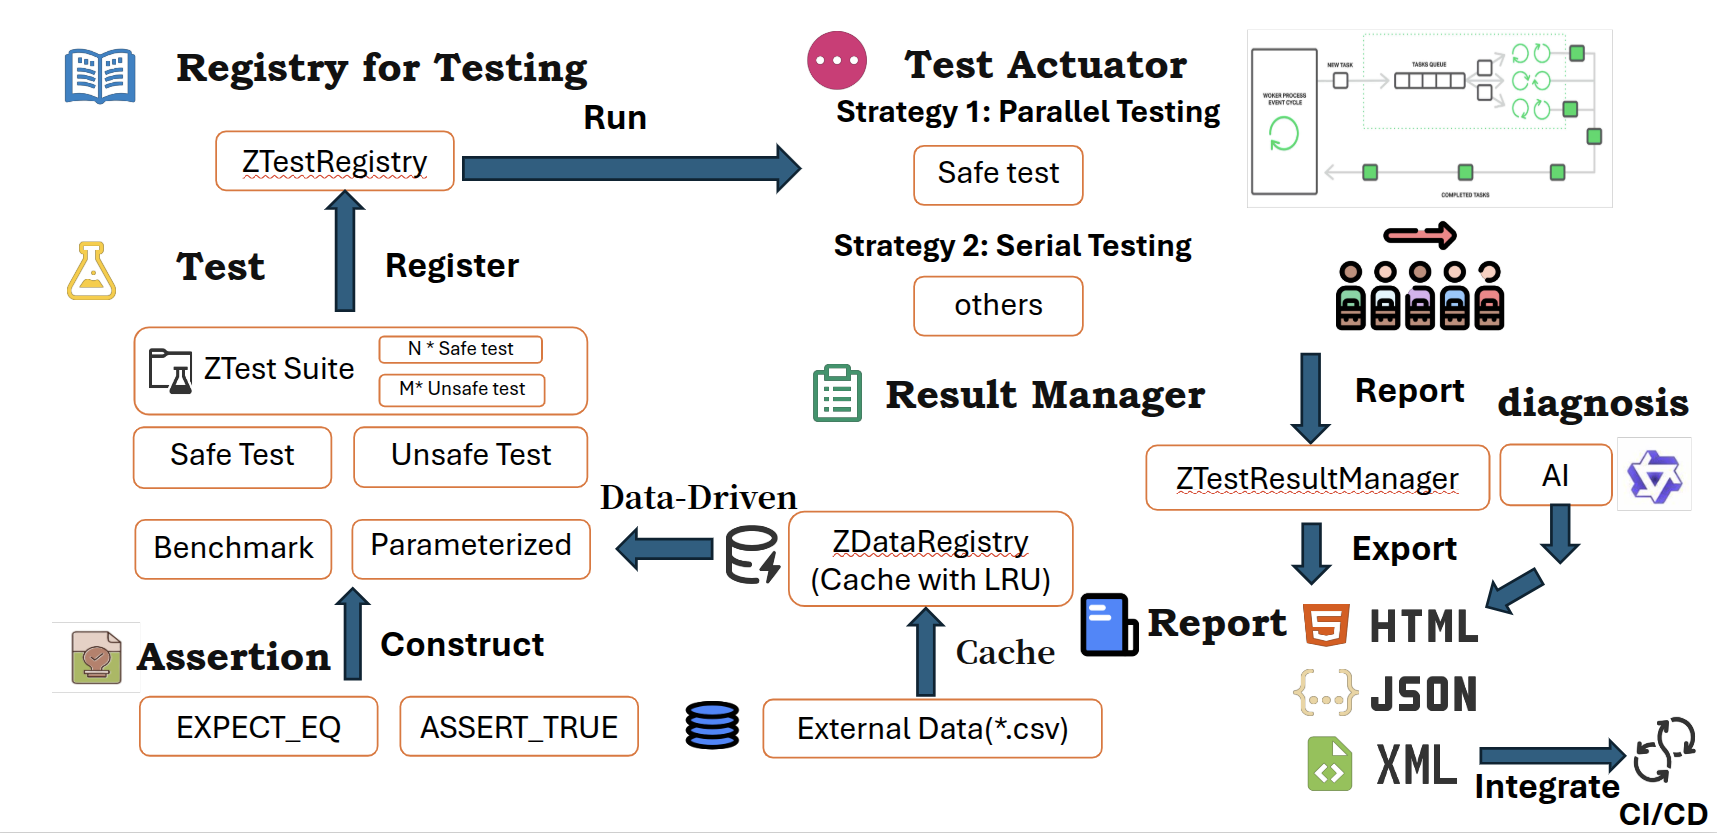
\includegraphics[width=0.8\textwidth]{img/core.png} % 假设logo.png是学校标志的图片文件
    \caption{ Ztest Design}
    \label{fig:ztest design }
\end{figure}
The core architecture of ZTest begins with the test definition phase, where tests (including ZTest Suite, safe tests, unsafe tests, benchmark tests, and parameterized tests) use assertions such as EXPECT\_EQ and ASSERT\_TRUE to validate the correctness of test results.
Next, tests are registered with ZTestRegistry for unified management.
After registration, tests are sent to the test executor, which adopts different test strategies based on the test type. Safe tests are executed using a parallel strategy, while other test types use a serial strategy.
During the execution of data-driven tests, the data-driven module manages external data (e.g., CSV files) through ZDataRegistry (a cache with LRU mechanism) to support test execution.
After testing completion, ZTestResultManager collects and processes test results and exports them in HTML, JSON, or XML formats for reporting and further analysis.
When exporting to HTML format, AI (qwen turbo) performs test diagnostics and integrates them into the HTML test report.
Additionally, the entire testing process supports integration with continuous integration/continuous deployment (CI/CD) systems, enabling automatic feedback of test results into the development workflow to enhance software development efficiency and quality.
\begin{figure}[H]
    \centering
    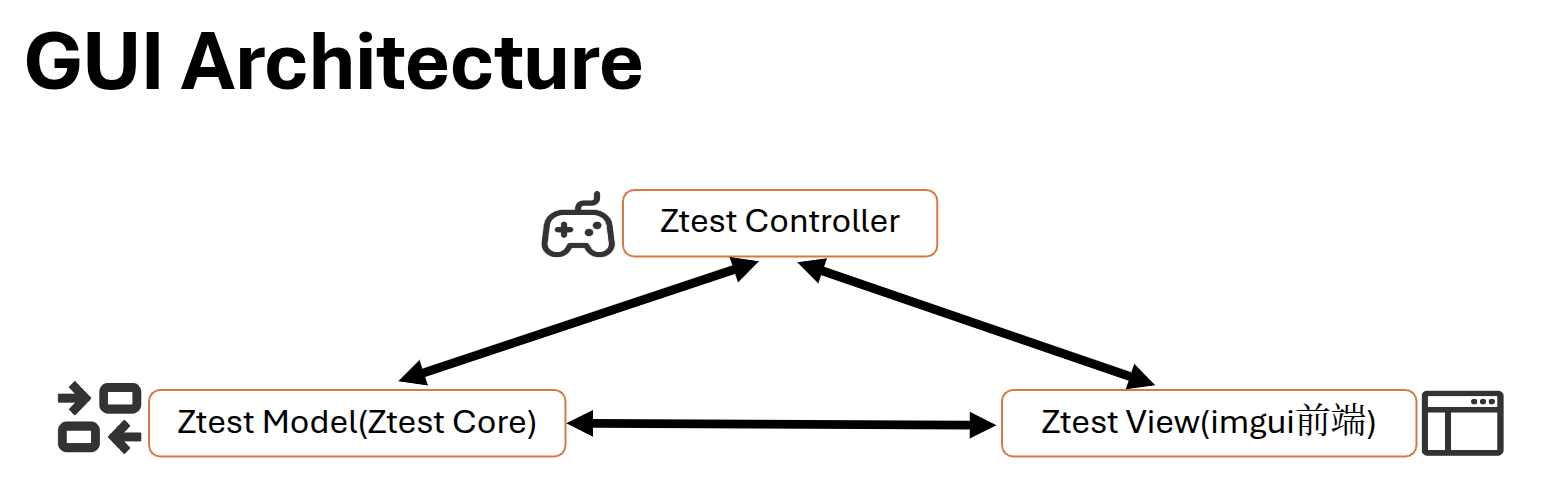
\includegraphics[width=0.8\textwidth]{img/guiarch.png} % 假设logo.png是学校标志的图片文件
    \caption{ Ztest GUI Architecture}
    \label{fig:ztest gui architecture }
\end{figure}
\subsubsection{GUI Framework}
The GUI framework is developed using the MVC architecture, where the Model layer handles data processing (further encapsulating Ztest core), the View layer is responsible for interface rendering (primarily using the ImGui framework), and the Controller layer manages user interactions. It translates user operations on the UI (such as clicks and filtering) into calls to the Model and View layers, thereby achieving updates to the user interface and data.
\subsubsection{Overall Class Diagram}
\begin{figure}[H]
    \centering
    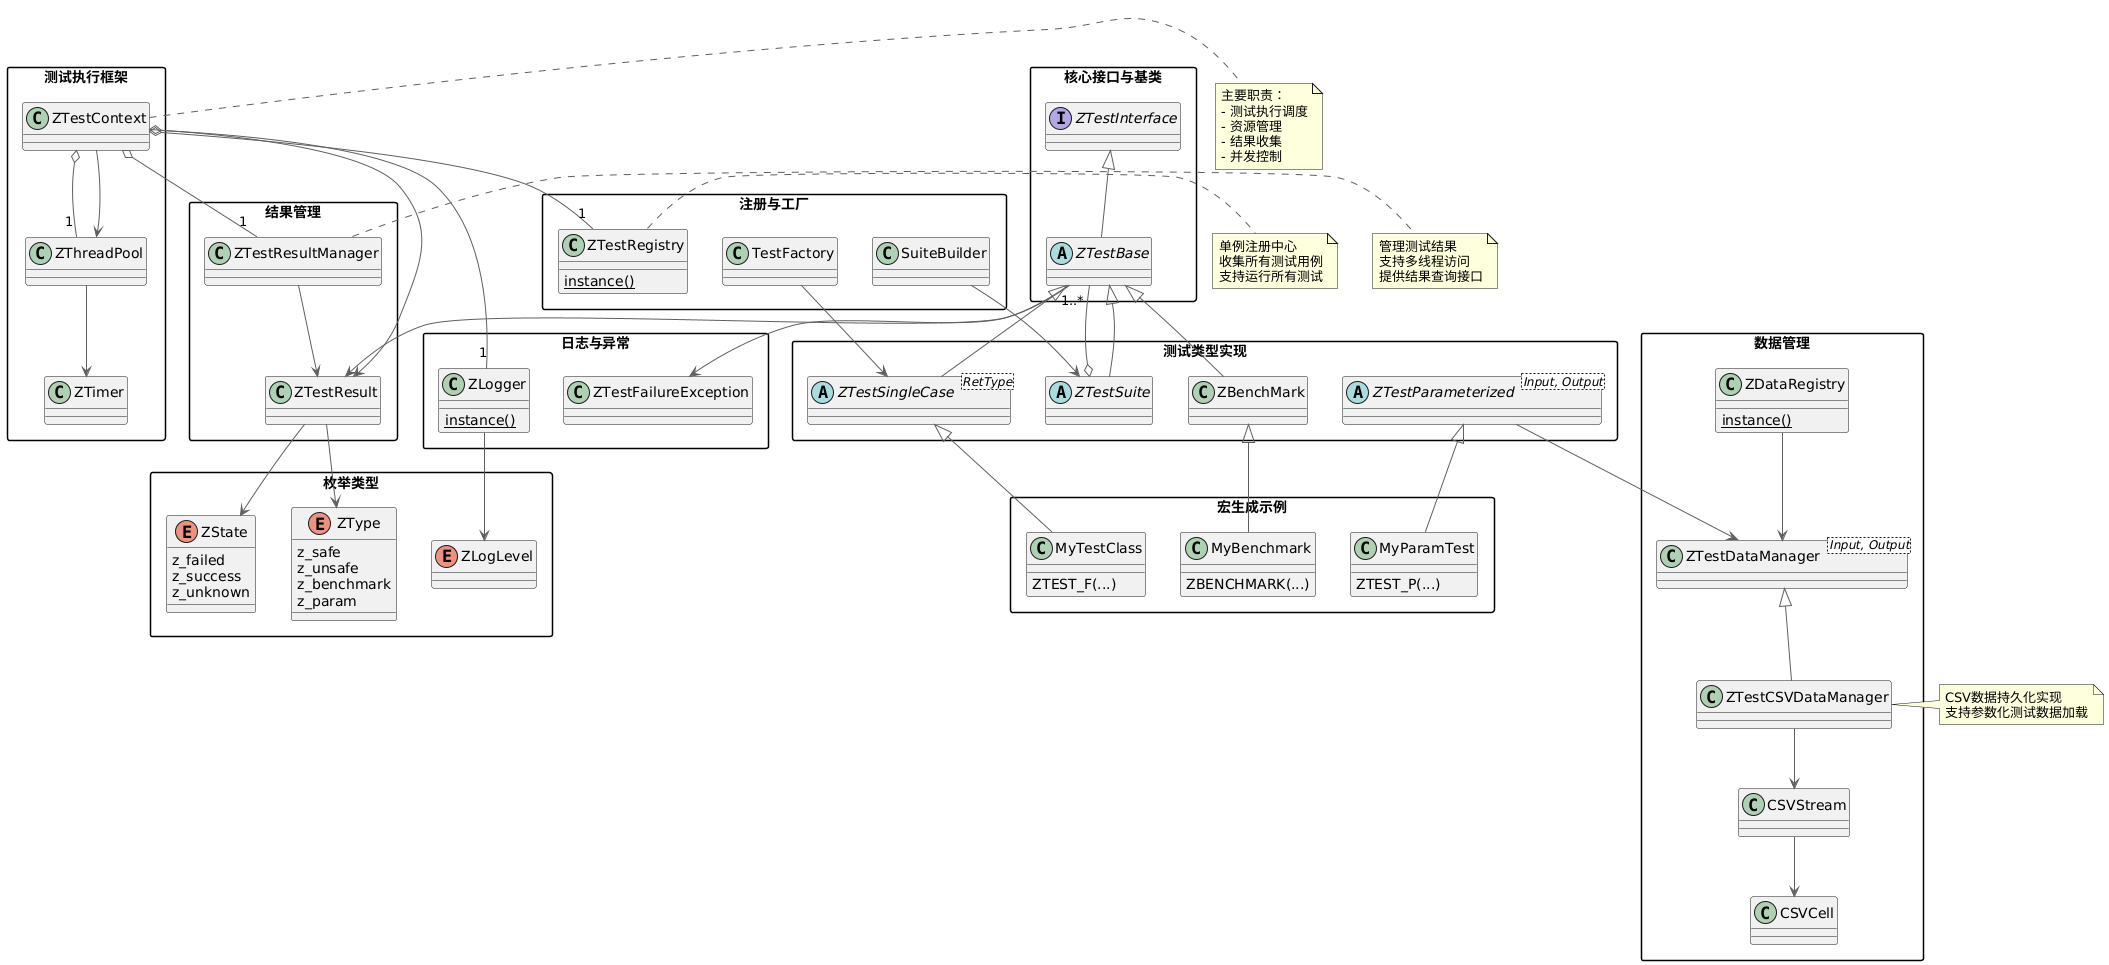
\includegraphics[angle=270,width=0.6\textwidth]{img/class.png} % 假设logo.png是学校标志的图片文件
    \caption{ Ztest Class}
    \label{fig:ztest class }
\end{figure}
\subsection{Detailed Design}
\subsubsection{Test Definition Related Classes}
\begin{itemize}
    \item \texttt{ZTestInterface}: Defines the test execution framework interface.
    \item \texttt{ZTestBase} (ztest\_base.hpp): An abstract base class for tests, encapsulating general properties and lifecycle hooks. It defines the test execution framework using the template method pattern, implements strategy pattern via virtual function tables, and extends using hook functions with decorator pattern characteristics.
    \item \texttt{ZTestSingleCase} (ztest\_singlecase.hpp): Implements single-case tests, executes test logic using the template method pattern, and demonstrates factory pattern usage with TestFactory, supporting chained configuration with builder pattern features.
    \item \texttt{ZTestSuite}(ztest\_suite.hpp): A test suite class inheriting from ZTestBase, implementing the template method pattern and supporting extension through hook functions.
    \item \texttt{ZBenchMark} (ztest\_benchmark.hpp): A benchmark test class inheriting from ZTestBase and overriding the run() method to implement benchmarking through iterative test function execution.
    \item \texttt{ZTestParameterized} (ztest\_parameterized.hpp): A base class for parameterized tests, encapsulating test data using the composite pattern and implementing a data-driven test framework through the run() method.
    \item \texttt{Macro Definition System} (ztest\_macros.hpp): Implements syntax sugar via macros, automatically generates test classes using the factory pattern, and achieves automatic registration with name concatenation techniques.
\end{itemize}
\begin{figure}[H]
    \centering
    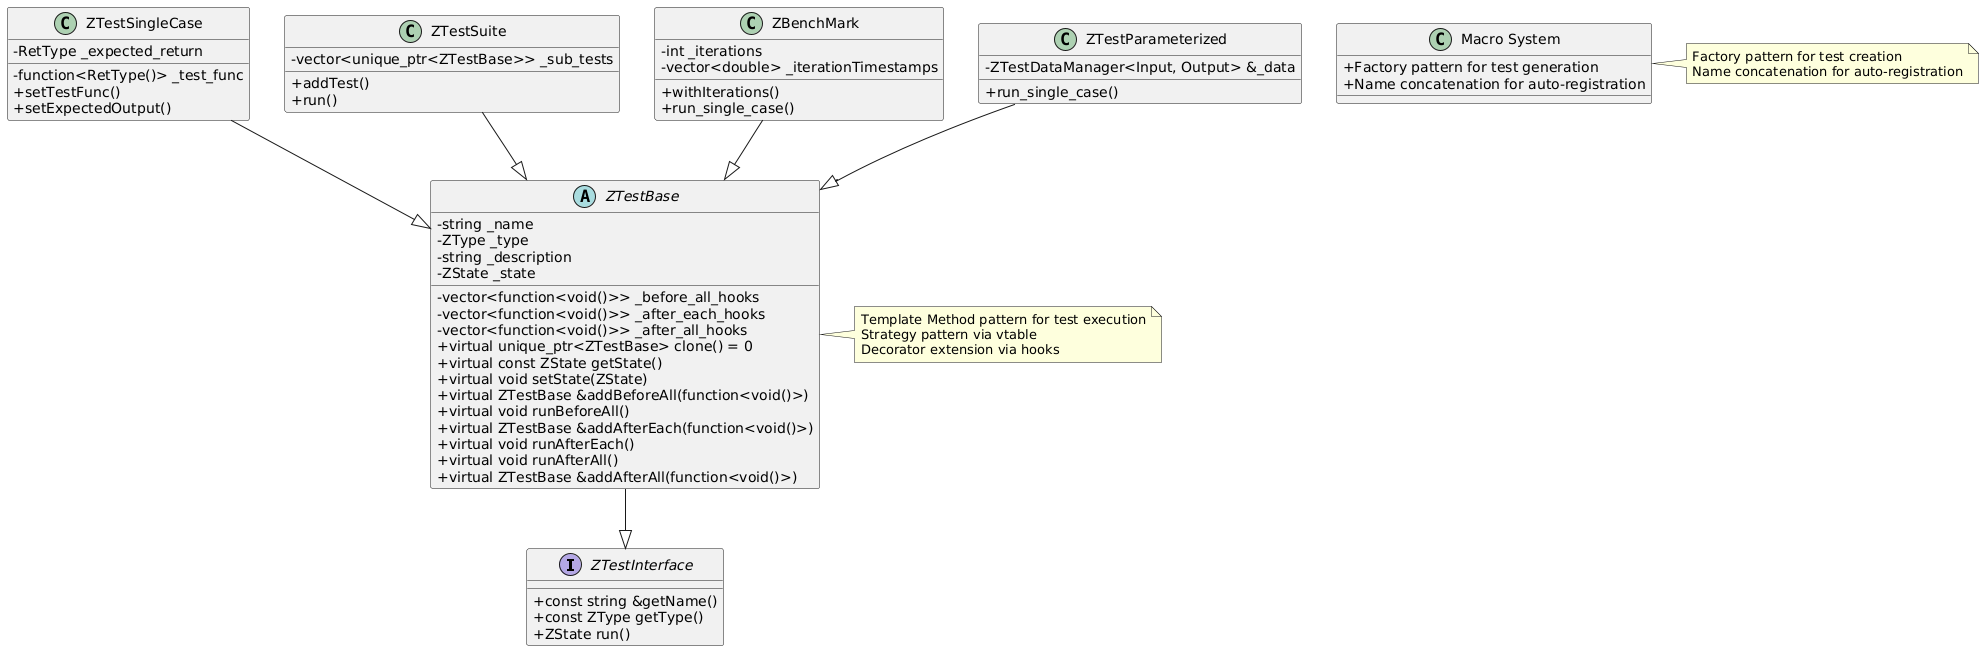
\includegraphics[width = \textwidth]{img/c1.png} % 假设logo.png是学校标志的图片文件
    \caption{ Ztest Class}
    \label{fig:ztest class }
\end{figure}

\subsubsection{Test Registration Related Classes}
\begin{itemize}
    \item \texttt{ZTestRegistry} (ztest\_registry.hpp): A globally accessible registry center implemented using the singleton pattern, managing test case collections and ensuring thread-safe registration and retrieval operations.
\end{itemize}
\begin{figure}[H]
    \centering
    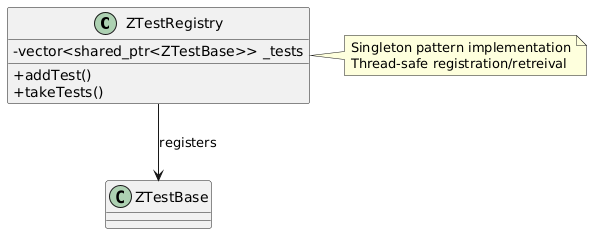
\includegraphics[width = 0.7\textwidth]{img/c2.png} % 假设logo.png是学校标志的图片文件
    \caption{ Ztest Class}
    \label{fig:ztest class }
\end{figure}
\subsubsection{Test Execution Related Classes}
\begin{itemize}
    \item \texttt{ZTestContext} (ztest\_context.hpp): A test execution context that selects execution strategies based on test types using the strategy pattern and implements parallel test execution via a thread pool.
    \item \texttt{ZThreadPool} (ztest\_thread.hpp): A thread pool implementing the object pool pattern, managing tasks using the producer-consumer model, and achieving asynchronous execution monitoring through future/promise mechanisms.
\end{itemize}
\begin{figure}[H]
    \centering
    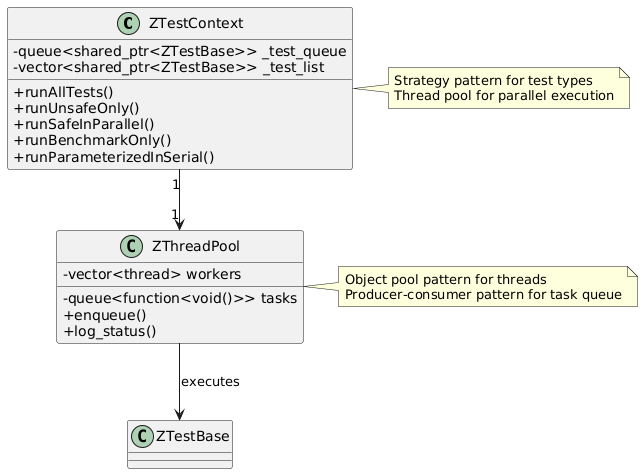
\includegraphics[width = 0.7\textwidth]{img/c3.png} % 假设logo.png是学校标志的图片文件
    \caption{ Ztest Class}
    \label{fig:ztest class }
\end{figure}
\subsubsection{Data Management Related Classes}
\begin{itemize}
    \item \texttt{ZDataRegistry} (ztest\_dataregistry.hpp): A data cache manager implemented using the singleton pattern for global access, with LRU strategy-based cache eviction.
    \item \texttt{ZDataManager}(ztest\_parameterized.hpp): An abstract base class for data management, providing data management interfaces and implementing iterator-like functionality similar to Python.
    \item \texttt{ZTestDataManager} (ztest\_parameterized.hpp): A generic class implementing test data management for user-specified data types.
    \item \texttt{ZTestCSVDataManager}(ztest\_parameterized.hpp): Inherits from \texttt{ZTestDataManager} and \texttt{ZDataManager}, implementing reading test data from CSV files and processing it into a format suitable for parameterized tests.
\end{itemize}
\begin{figure}[H]
    \centering
    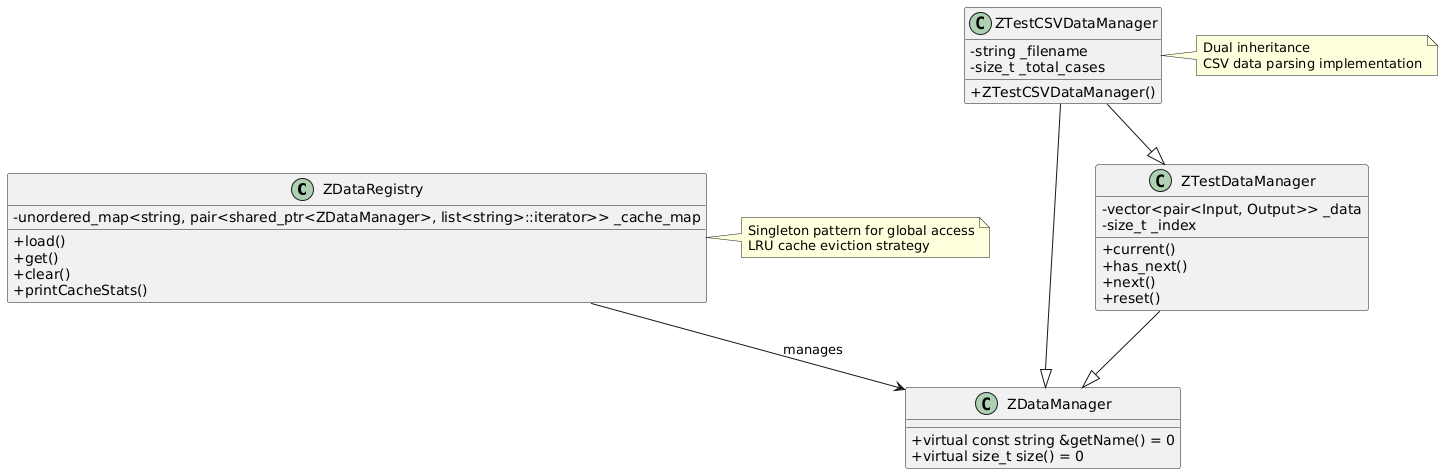
\includegraphics[width = \textwidth]{img/c4.png} % 假设logo.png是学校标志的图片文件
    \caption{ Ztest Class}
    \label{fig:ztest class }
\end{figure}
\subsubsection{Result Management Related Classes}
\begin{itemize}
    \item \texttt{ZTestResult} (ztest\_result.hpp): A value object pattern-based test result class encapsulating immutable data such as test status and duration.
    \item \texttt{ZTestResultManager} (ztest\_result.hpp): A result manager implemented using the singleton pattern, handling result storage and queries via the chain of responsibility pattern.
\end{itemize}
\begin{figure}[H]
    \centering
    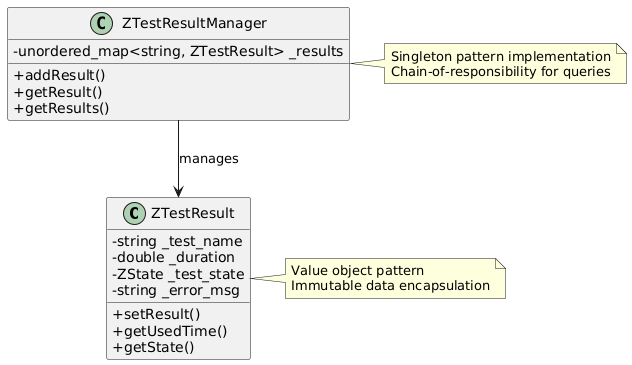
\includegraphics[width = 0.7\textwidth]{img/c5.png} % 假设logo.png是学校标志的图片文件
    \caption{ Ztest Class}
    \label{fig:ztest class }
\end{figure}
\subsubsection{Report Generation Related Classes}
\begin{itemize}
    \item \texttt{ZLogger} (ztest\_logger.hpp): A multi-format report generator applying the template method pattern to define the report generation process and supporting HTML, JSON, and JUnit report formats.
\end{itemize}
\begin{figure}[H]
    \centering
    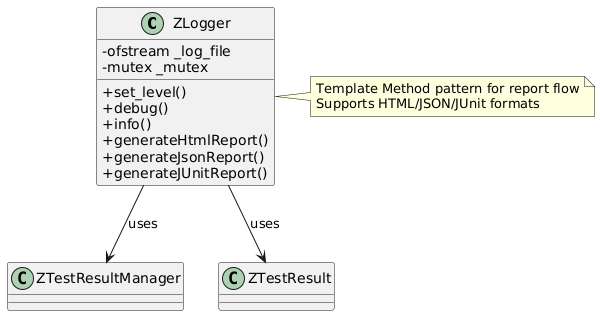
\includegraphics[width =0.7\textwidth]{img/c6.png} % 假设logo.png是学校标志的图片文件
    \caption{ Ztest Class}
    \label{fig:ztest class }
\end{figure}
\subsubsection{Utility Module Related Classes}
\begin{itemize}
    \item \texttt{ZTimer} (ztest\_timer.hpp): A timer implementing the RAII pattern for time measurement.
    \item \texttt{CSVStream}(ztest\_utils.hpp): Implements CSV stream operations similar to standard input/output libraries, supporting read, write, and basic information printing.
\end{itemize}
\begin{figure}[H]
    \centering
    \includegraphics[width = \textwidth]{img/c7.png} % 假设logo.png是学校标志的图片文件
    \caption{ Ztest Class}
    \label{fig:ztest class }
\end{figure}
\subsubsection{GUI Module Related Classes}
\begin{itemize}
    \item \texttt{ZTestModel} (gui.hpp): The Model layer in the MVC architecture, implementing the observer pattern to listen for test status changes.
    \item \texttt{ZTestController} (gui.hpp): The Controller layer in the MVC architecture, encapsulating test execution operations using the command pattern.
    \item \texttt{ZTestView} (gui.hpp): The View layer in the MVC architecture, employing the bridge pattern to separate interface elements from their implementation.
\end{itemize}
\begin{figure}[H]
    \centering
    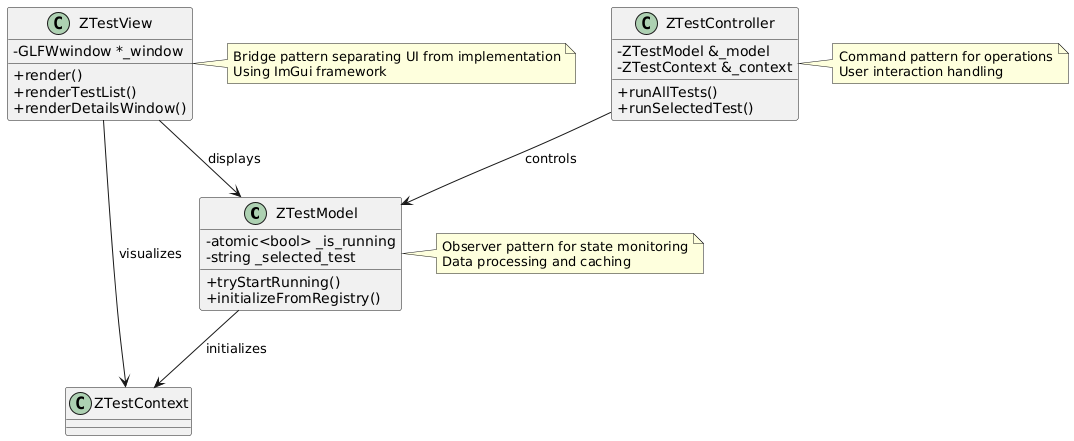
\includegraphics[width = \textwidth]{img/c8.png} % 假设logo.png是学校标志的图片文件
    \caption{ Ztest Class}
    \label{fig:ztest class }
\end{figure}
\section{Programming Progress}
\begin{table}[H]
    \centering
    \begin{tabular}{|l|l|}
        \toprule
        \textbf{Task Phase}                                           & \textbf{Plan}                                                       \\ \midrule
        \textbf{Theme Confirmation} 2024.04.26-2024.05.03             & Investigate themes and submit proposals.                            \\ \midrule
        \textbf{Core Code Implementation} 2024.05.03-2024.05.05       & Implemented GUI and execution logic for Safe test and Unsafe test   \\ \midrule
        \textbf{Major Performance Optimization} 2024.05.05-2024.05.08 & Thread pool optimization                                            \\ \midrule
        Feature Optimization 2024.05.08-2024.05.11                    & Improved JSON, HTML output, JUnit format output, and CI integration \\ \midrule
        Feature Optimization 2024.05.11-2024.05.13                    & Introduced imgui Docking functionality in GUI                       \\ \midrule
        Feature Optimization 2024.05.13-2024.05.15                    & Added CLI                                                           \\ \midrule
        \textbf{Major Feature Optimization} 2024.05.15-2024.05.24     & Added BENCHMARK testing                                             \\ \midrule
        Feature Optimization 2024.05.24-2024.05.25                    & Added device status monitoring and visualization                    \\ \midrule
        \textbf{Major Feature Optimization} 2024.05.25-2024.05.28     & Added parameterized testing and data-driven support                 \\ \midrule
        \textbf{Major Performance Optimization} 2024.05.28-2024.06.02 & Implemented data caching and LRU cache eviction technology          \\ \midrule
        \textbf{Major Feature Optimization}  2024.06.02-2024.06.07    & Added AI diagnostics                                                \\ \midrule
        Summary Work 2024.6.02-2024.06.08                             & Cross-platform migration \& report writing                          \\
        \bottomrule
    \end{tabular}
    \caption{Programming Progress}
\end{table}

\section{Test Report}
\subsection{Function Testing \& System Testing}
\subsubsection{Assertion Function Testing}
This test aims to verify the behavior of assertion macros such as EXPECT\_EQ, EXPECT\_NEAR, and ASSERT\_TRUE in both successful and failed scenarios. By designing different test cases, it checks whether these assertions can correctly identify matches between expected and actual results, ensuring the reliability of the testing framework's assertion functionality.
\begin{framed}
    \begin{lstlisting}[language=C++]
int add(int a, int b) { return a + b; }
double subtract(double a, double b) { return a - b; }
ZTEST_F(ASSERTION, FailedEXPECT_EQ) {
  EXPECT_EQ(6, add(2, 3));
  return ZState::z_success;
}
ZTEST_F(ASSERTION, SuccessEXPECT_EQ) {
  EXPECT_EQ(5, add(2, 3));
  return ZState::z_success;
}
ZTEST_F(ASSERTION, SuccessEXPECT_NEAR) {
  EXPECT_NEAR(2, subtract(5.0, 3.0), 0.001);
  return ZState::z_success;
}

ZTEST_F(ASSERTION, FailedEXPECT_NEAR) {
  EXPECT_NEAR(2, subtract(5.1, 3.0), 0.001);
  return ZState::z_success;
}

ZTEST_F(ASSERTION, FailedASSERT_TRUE) {
  ASSERT_TRUE(false);
  return ZState::z_success;
}
ZTEST_F(ASSERTION, SuccessASSERT_TRUE) {
  ASSERT_TRUE(true);
  return ZState::z_success;
}
\end{lstlisting}
\end{framed}
\begin{figure}[H]
    \centering
    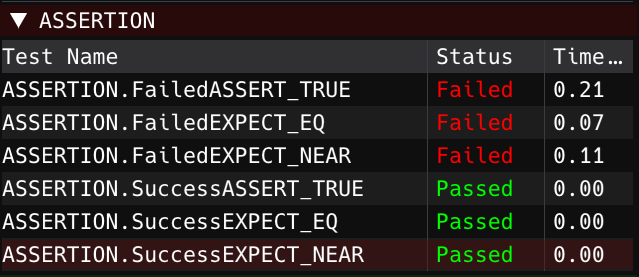
\includegraphics[width=0.7\textwidth]{img/ass.png} % 假设logo.png是学校标志的图片文件
    \caption{Assertion Function Test}
    \label{fig:assertion function test}
\end{figure}
\subsubsection{Test Management Testing}
This test module aims to verify the completeness and reliability of the test management system. By defining various test cases, including single safe tests, single unsafe tests, and test suites with multiple assertions, the system comprehensively covers different testing scenarios. Additionally, dynamic test case construction allows for flexible creation and registration of new test cases, enhancing the test framework's extensibility. During testing, memory allocation, function calls, and assertion checks ensure the correct execution of test cases and consistency with expected results. The test framework also provides pre and post hooks for necessary setup and cleanup operations before and after tests, ensuring test environment stability and result accuracy.
\begin{framed}
    \begin{lstlisting}[language=C++]
ZTEST_F(TESTMANAGE, safe_test_single_case, safe) {
  ASSERT_TRUE(true);
  return ZState::z_success;
}
ZTEST_F(TESTMANAGE, unsafe_test_single_case, unsafe) {
  ASSERT_TRUE(true);
  return ZState::z_success;
}
ZTEST_F(TESTMANAGE, test_suite) {
  const size_t MB100 = 100 * 1024 * 1024;
  auto ptr = std::make_unique<char[]>(MB100);
  ASSERT_TRUE(ptr != nullptr);
  EXPECT_EQ(3, subtract(5, 3));
  EXPECT_EQ(6, add(2, 3));
  return ZState::z_success;
}
void createSingleTestCase() {
  // Use TestBuilder to construct test
  auto test =
      TestFactory::createTest("AdditionTest",                // Test name
                              ZType::z_safe,                 // Execution
                              "Test addition functionality", // Description
                              add, 2, 3 // Function and arguments
                              )
          .setExpectedOutput(5) // Set expected result
          .beforeAll([]() {     // Setup hook
            std::cout << "Setting up single test..." << std::endl;
          })
          .afterEach([]() { // Teardown hook
            std::cout << "Cleaning up after test..." << std::endl;
          })
          .withDescription("Verify basic addition")
          .registerTest()
          .build(); // Register with test
}
// in main()
createSingleTestCase();

\end{lstlisting}
\end{framed}
\begin{figure}[H]
    \centering
    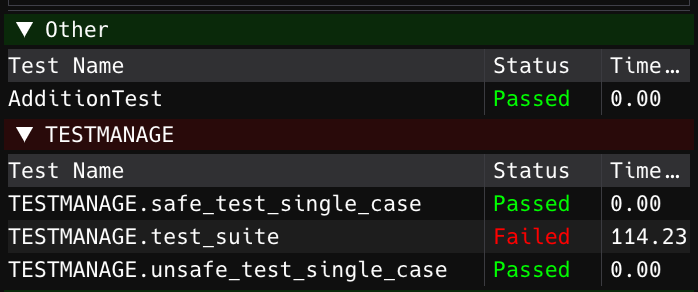
\includegraphics[width=0.7\textwidth]{img/manage.png} % 假设logo.png是学校标志的图片文件
    \caption{Test Management Function Test}
    \label{fig:test management function test}
\end{figure}
\newpage
\subsubsection{Test Execution Management}
This test module primarily verifies the efficiency and accuracy of the test execution management mechanism. Multiple safe and unsafe test cases are defined to simulate different execution times and task types. Each test case simulates varying execution times using the sleep function to evaluate the performance differences between parallel and sequential execution.
Test results are interpreted as follows:
\begin{itemize}
    \item A thread pool with eight threads is used to execute three test cases in parallel.
    \item Three test cases are executed sequentially.
\end{itemize}
\begin{framed}
    \begin{lstlisting}[language=C++]
ZTEST_F(RUN, safe_test_single_case1, safe) {
  sleep(2);
  ASSERT_TRUE(true);
  return ZState::z_success;
}
ZTEST_F(RUN, safe_test_single_case2, safe) {
  sleep(1);
  ASSERT_TRUE(true);
  return ZState::z_success;
}
ZTEST_F(RUN, safe_test_single_case3, safe) {
  sleep(3);
  ASSERT_TRUE(true);
  return ZState::z_success;
}
ZTEST_F(RUN, unsafe_test_single_case1, unsafe) {
  sleep(1);
  EXPECT_EQ(false, false);
  return ZState::z_success;
}
ZTEST_F(RUN, unsafe_test_single_case2, unsafe) {
  sleep(2);
  EXPECT_EQ(false, false);
  return ZState::z_success;
}
ZTEST_F(RUN, unsafe_test_single_case3, unsafe) {
  sleep(3);
  EXPECT_EQ(false, false);
  return ZState::z_success;
}
\end{lstlisting}
\end{framed}
\begin{figure}[H]
    \centering
    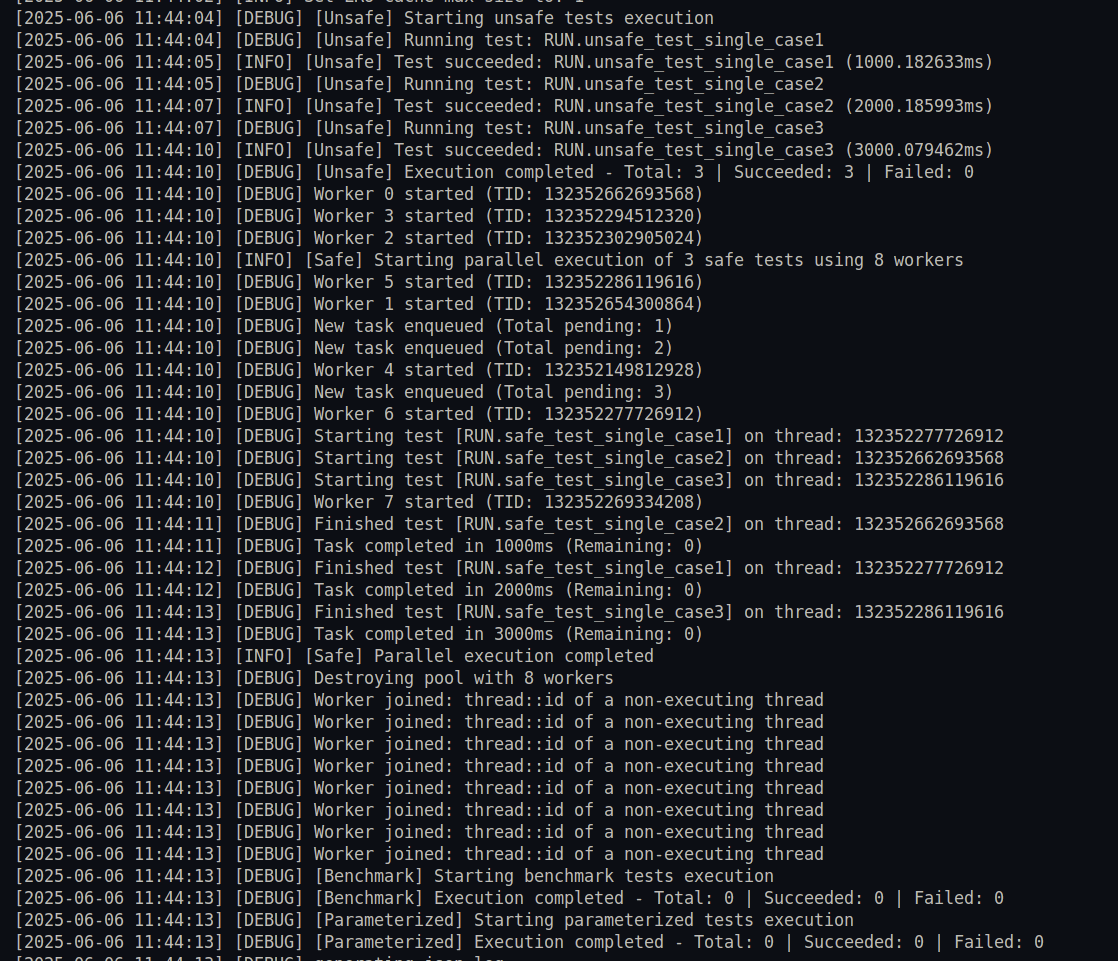
\includegraphics[width=\textwidth]{img/context.png}
    \caption{Test Executor Function Test}
    \label{fig:test executor function test}
\end{figure}

\subsubsection{Data-Driven Testing}
Two types of data-driven test cases are demonstrated, utilizing in-memory datasets and external CSV files as data sources.

\begin{framed}
    \begin{lstlisting}[language=C++]
ZTestDataManager<vector<int>, int> sum_test_data = {
    {{1, 2}, 3}, {{-1, 1}, 0}, {{10, 20}, 30}};
ZTEST_P(ArithmeticSuite, SumTest, sum_test_data) {
  auto &&[inputs, expected] = _data.current();
  int actual = inputs[0] + inputs[1];
  EXPECT_EQ_FOREACH(expected, actual);
  return ZState::z_success;
}
ZTestDataManager<tuple<float, int>, float> sum_test_data2 = {
    {{1.2, 2}, 3.2}, {{-1.0, 1}, 0.0}, {{10.1, 20}, 30.2}};
ZTEST_P(ArithmeticSuite, SumTestfordiff, sum_test_data2) {
  auto &&[inputs, expected] = _data.current();
  float actual = std::get<0>(inputs) + std::get<1>(inputs);
  EXPECT_EQ_FOREACH(expected, actual);
  return ZState::z_success;
}
ZTEST_P_CSV(MathTests, AdditionTests, "data.csv") {
  auto inputs = getInput();
  auto expected = getOutput();
  double actual = std::get<double>(inputs[0]) + std::get<double>(inputs[1]);
  EXPECT_EQ(actual, std::get<double>(expected));
  return ZState::z_success;
}
\end{lstlisting}
\end{framed}
\begin{figure}[H]
    \centering
    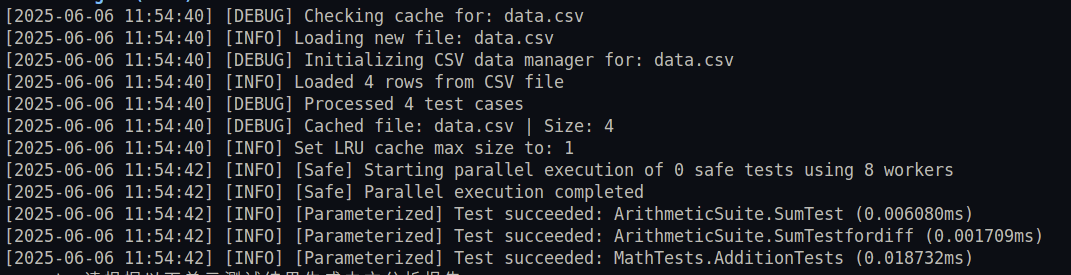
\includegraphics[width=\textwidth]{img/data.png}
    \caption{Data-Driven Function Test}
    \label{fig: Data-Driven Function Test}
\end{figure}
\subsubsection{Benchmark Testing}
Testing the definition of benchmark-type tests, visualizing test time distribution, and monitoring CPU and memory usage in the GUI.

\begin{framed}

    \begin{lstlisting}[language=C++]
ZBENCHMARK(Vector, PushBack) {
  std::vector<int> v;
  for (int i = 0; i < 10000; ++i)
    v.push_back(i);
  return ZState::z_success;
}
ZBENCHMARK(Matrix, PushBack, 20000) {
  std::vector<int> v;
  for (int i = 0; i < 1000; ++i)
    v.push_back(random());
  return ZState::z_success;
}\end{lstlisting}
\end{framed}
\begin{figure}[H]
    \centering
    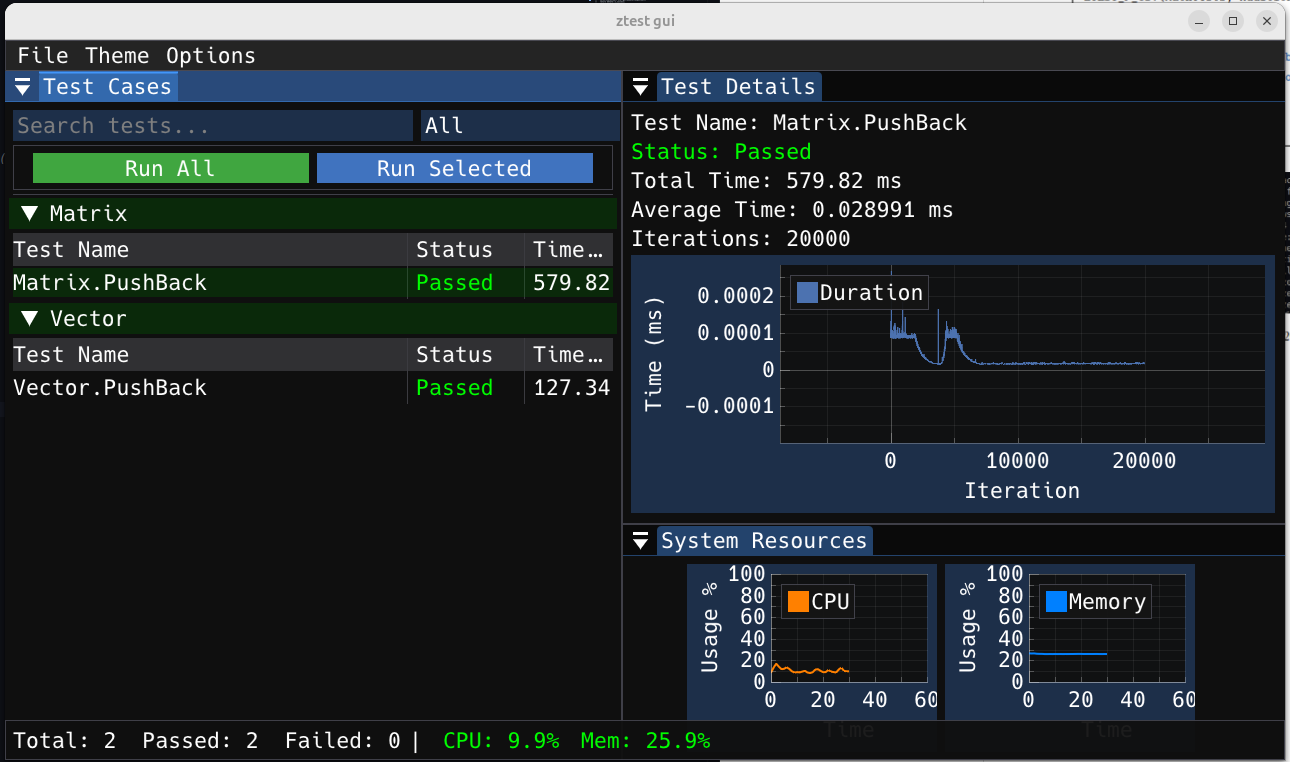
\includegraphics[width=\textwidth]{img/ben.png}
    \caption{Data-Driven Function Test}
    \label{fig: Data-Driven Function Test}
\end{figure}

\begin{itemize}
    \item
\end{itemize}
\subsubsection{Report Generation Testing}

Testing the generation of HTML, JSON, and XML formatted reports.
\begin{figure}[H]
    \centering
    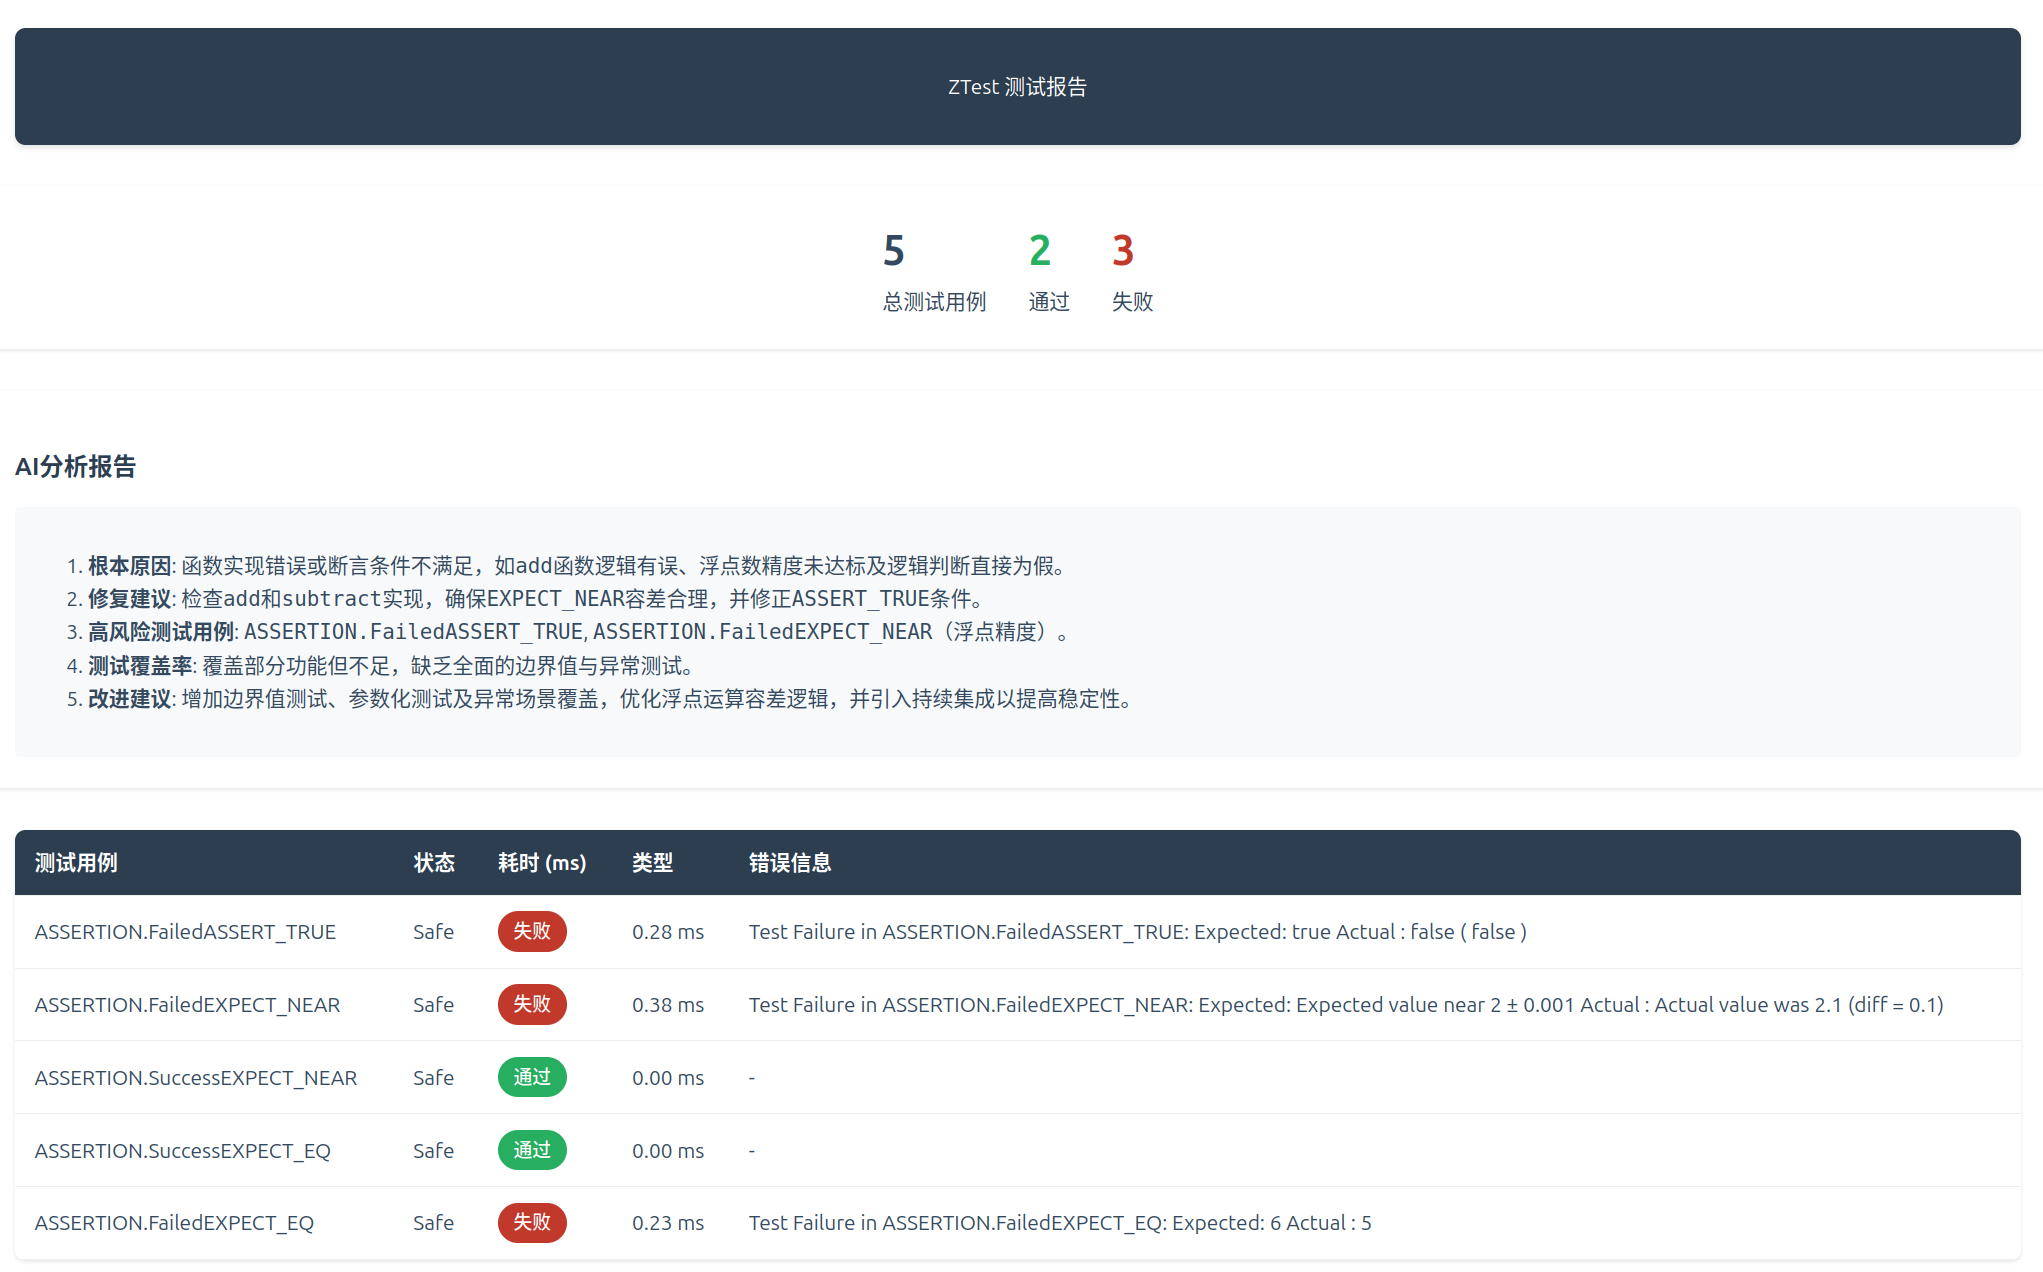
\includegraphics[width=0.8\textwidth]{img/html.png}
    \caption{HTML Test Report}
    \label{fig: Data-Driven Function Test}
\end{figure}
\begin{figure}[H]
    \centering
    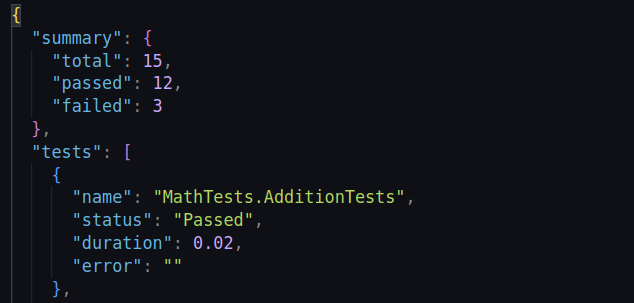
\includegraphics[width=0.6\textwidth]{img/json.png}
    \caption{Partial JSON Report}
    \label{fig: Data-Driven Function Test}
\end{figure}

\begin{figure}[H]
    \centering
    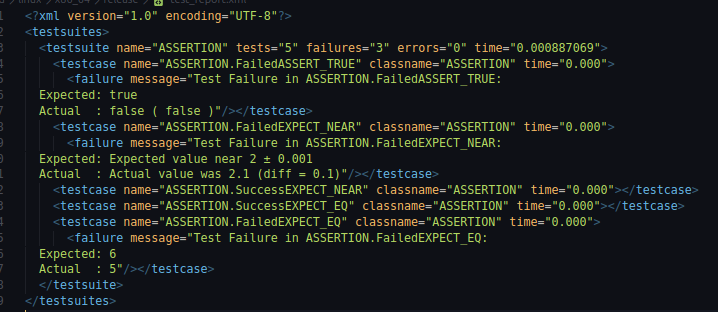
\includegraphics[width=0.6\textwidth]{img/xml.png}
    \caption{XML (JUnit Format) Report}
    \label{fig: Data-Driven Function Test}
\end{figure}
\subsubsection{GUI Testing}
Testing the GUI display, theme switching, AI assistant display, and other functionalities.
\begin{figure}[H]
    \centering
    \begin{minipage}{0.5\textwidth}
        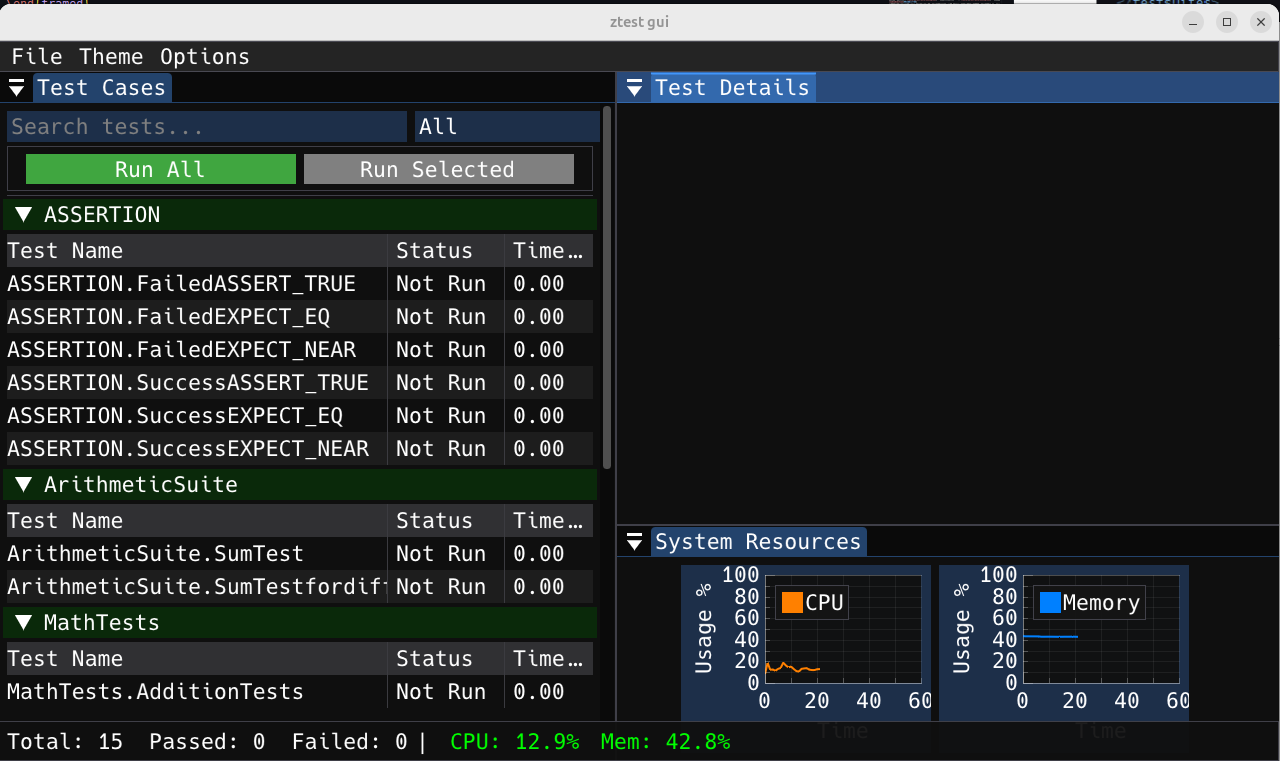
\includegraphics[width=\textwidth]{img/showgui.png}
        \caption{Dark Theme GUI Display}
        \label{fig:showgui}
    \end{minipage}%
    \begin{minipage}{0.5\textwidth}
        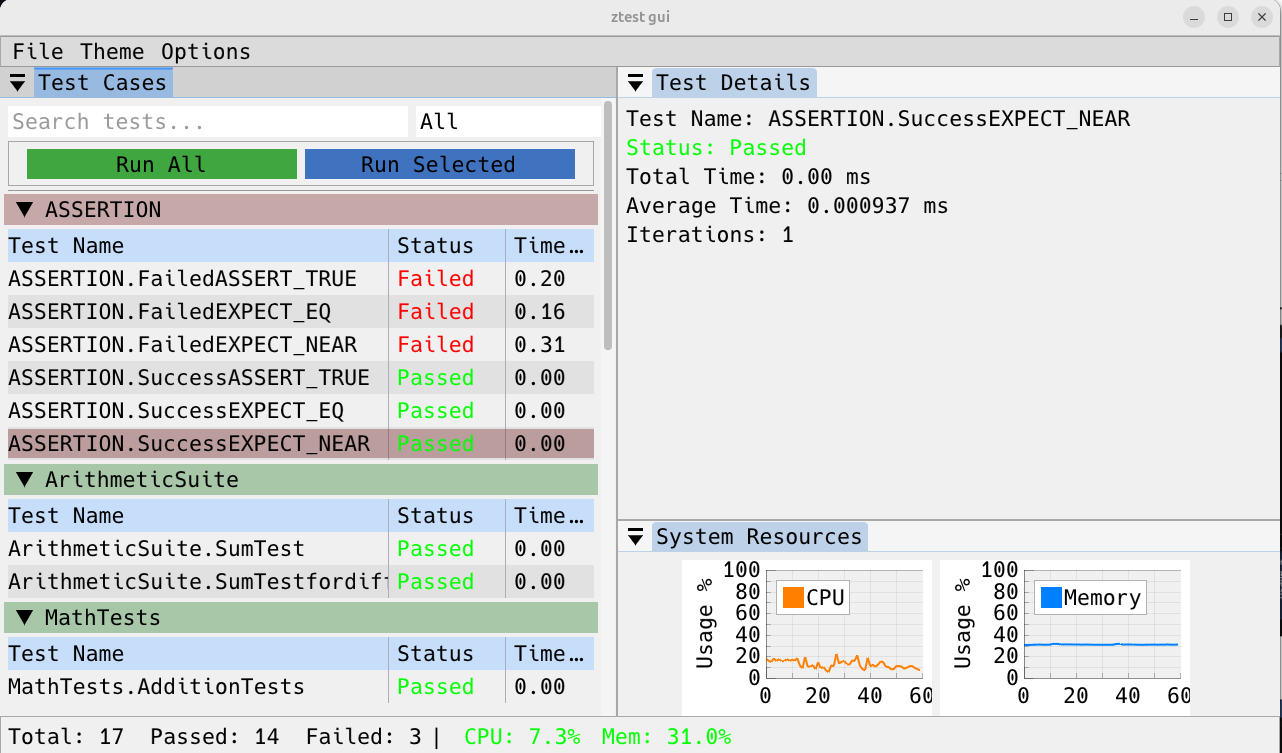
\includegraphics[width=\textwidth]{img/light.png}
        \caption{Light Theme GUI Display}
        \label{fig:light}
    \end{minipage}
\end{figure}
\begin{figure}[H]
    \centering
    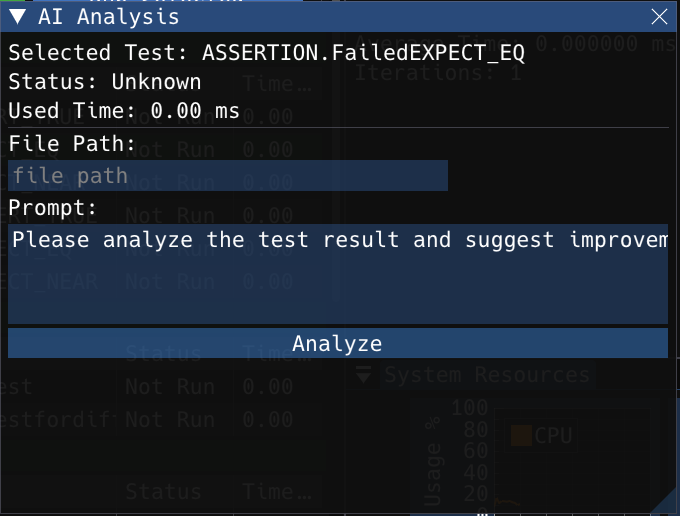
\includegraphics[width=0.4\textwidth]{img/aih.png}
    \caption{AI Diagnostic Assistant Display}
    \label{fig: Data-Driven Function Test}
\end{figure}
\subsubsection{AI Diagnosis Testing}
During report generation, AI (qwen turbo) is invoked for diagnostics and integrated into the HTML report.
\begin{figure}[H]
    \centering
    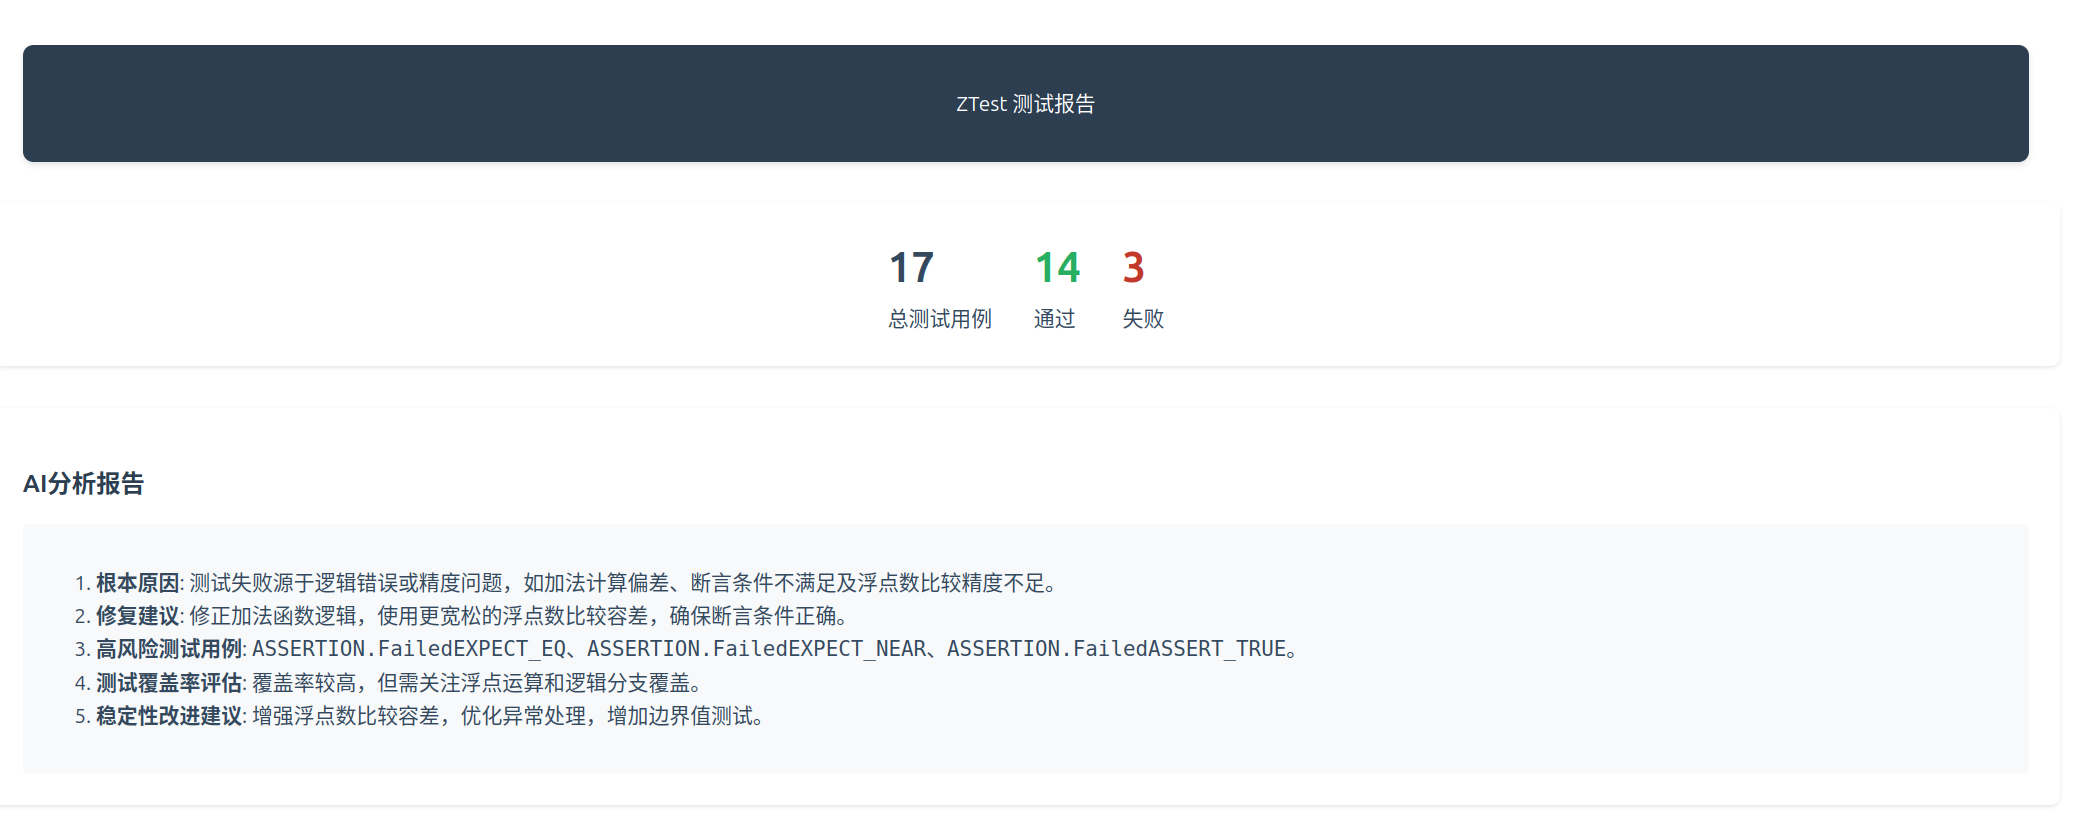
\includegraphics[width=\textwidth]{img/ai.png}
\end{figure}
In the GUI interface, AI (qwen turbo) is called to diagnose individual test cases and display results, allowing users to input custom prompts and file paths.
\begin{figure}[H]
    \centering
    \begin{minipage}{0.45\textwidth}
        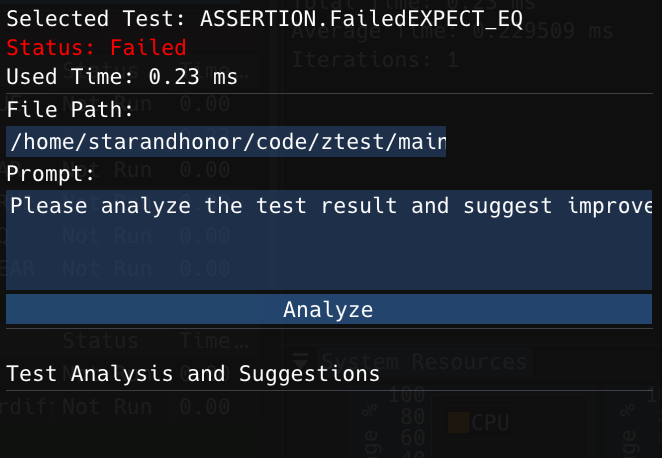
\includegraphics[width=\textwidth]{img/aih1.png}
    \end{minipage}
    \hfill
    \begin{minipage}{0.45\textwidth}
        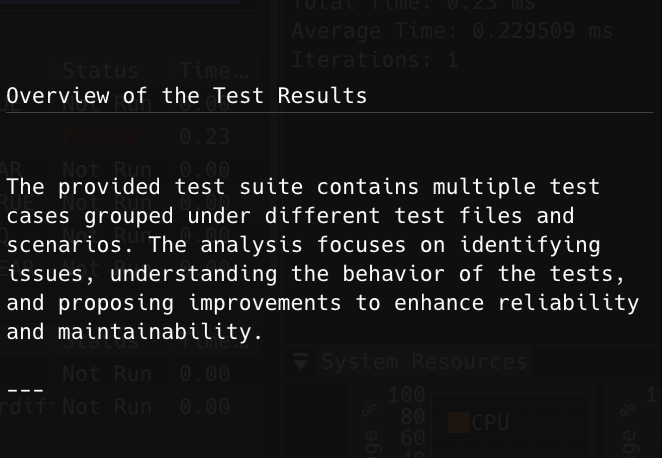
\includegraphics[width=\textwidth]{img/aih2.png}
    \end{minipage}
\end{figure}


\section{Personal Summaries}
\begin{tabular}{|p{50pt}|p{350pt}|}
    \hline
    Name           & Summary                                                                                                                                                                                                                                                                                                                                                                                                                                                                                                                                                                                                                                                                                                                                                                                                                                                                                                                                                                                                                                                                                                                                                                                                                      \\ \hline
    Zheng Chenyang & During the test framework design and implementation process, I deeply appreciated the importance of modular design and layered architecture. By introducing the MVC pattern, I achieved a clear separation of models, views, and controllers, enhancing code maintainability and extensibility. In a multithreaded environment, I optimized resource monitoring and task scheduling, ensuring system stability and performance. Additionally, by integrating AI analysis capabilities, I provided intelligent feedback for test results, enhancing the tool's utility. The development process strengthened my technical expertise and made me more mindful of teamwork and communication efficiency. In the future, I will continue to iterate, refine features, and improve user experience.                                                                                                                                                                                                                                                                                                                                                                                                                               \\ \hline
    Ye Suohua      & In this program, I was mainly responsible for the frontend part, choosing the imgui library for frontend development and successfully completing the frontend architecture and rendering. I realized that frontend structures need to be designed based on user requirements, considering factors such as cross-platform compatibility and library version issues.                                                                                                                                                                                                                                                                                                                                                                                                                                                                                                                                                                                                                                                                                                                                                                                                                                                           \\ \hline
    Qi Yansong     & Participating in the development of the "ztest" unit testing framework, I felt that the knowledge I learned could be applied not only to game development but also to tool software design. As a lightweight and easy-to-use C++ testing framework, ztest addresses the shortcomings of existing frameworks like Google Test in terms of GUI support, concurrent testing, and reporting systems. Through innovative design, it enhances user experience and extensibility. I particularly appreciated the team's implementation of multiple test case creation methods, which reflect the "user-friendly" design philosophy. The design of multithreaded safety evaluations made me aware of the complexity of concurrency issues and the importance of categorized handling. Through practice, I gained a deeper understanding of modern C++ features and design patterns. This experience not only improved my technical skills but also made me recognize that excellent software products need to balance technical depth with user experience. Efficient team communication and collaboration are key to achieving this, and I look forward to continuing to explore challenges and solutions in engineering practices. \\ \hline
    Wang Ruizhen   & Through this project, I have grown a lot. It was a large-scale project with a high degree of complexity, posing a significant challenge for me. Due to time constraints, I had to learn on the job. Although it was rushed and I only had a superficial understanding of many aspects, I also gained a wealth of knowledge, mastered new skills, and honed my problem-solving abilities.                                                                                                                                                                                                                                                                                                                                                                                                                                                                                                                                                                                                                                                                                                                                                                                                                                     \\ \hline
    Wu Hongqing    & In the zTest project, I was responsible for GUI design. On the technical side, I gained practical experience in applying the MVC architecture, utilized the ImGui framework to create a visual interface, designed a simple visualization window, and coordinated the ZTestModel, ZTestView, and ZTestController classes to handle data visualization, thereby enhancing user-friendliness. In terms of teamwork, I improved my collaboration skills by working with the team to define interfaces and advance the project. I also standardized the implementation of different classes within the project to prevent compilation errors and reduce the difficulty of understanding for team members.                                                                                                                                                                                                                                                                                                                                                                                                                                                                                                                        \\ \hline
\end{tabular}

\section{References}
\begin{thebibliography}{99}
    \bibitem{gtest} Google Test. \textit{Google Test Documentation}. [Online]. Available: https://github.com/google/googletest
    \bibitem{junit} JUnit. \textit{JUnit Documentation}. [Online]. Available: https://junit.org/junit5/
    \bibitem{catch} Catch2. \textit{Catch2 Documentation}. [Online]. Available: https://github.com/catchorg/Catch2
    \bibitem{gtest-parallel} Google Test Parallel. \textit{Google Test Parallel Documentation}. [Online]. Available: https://github.com/google/gtest-parallel
    \bibitem{pytest} Pytest. \textit{Pytest Documentation}. [Online]. Available: https://docs.pytest.org/en/latest/
    \bibitem{miniunit} MiniUnit. \textit{MiniUnit Documentation}. [Online]. Available: https://github.com/urin/miniunit
\end{thebibliography}

\end{document}